\documentclass{beamer}
\RequirePackage{luatex85}
\include{../style/cours-style.sty}

% Title
\title{Data Security - Bachelor CSI}
\author{Christophe Brun}
\institute{Campus Saint-Michel IT}
\date{25 juin 2024}
\beamertemplatenavigationsymbolsempty

\titlegraphic{
    \bigbreak
    
\includegraphics[width=2cm]{image/logo-papit}
    
\includegraphics[width=2cm]{image/logo-campus-saint-michel-it}
}
\begin{document}

    \begin{frame}
        \titlepage
        \bigbreak
        \centering
        \url{https://github.com/St-Michel-IT/data-security/}
    \end{frame}

    \begin{frame}{Table des matières}
        \begin{multicols}{2}
            \tableofcontents
        \end{multicols}
    \end{frame}


    \section{Programme du module}\label{sec:programme-du-module}
    \begin{frame}{Data Security}{Compétences}
        \begin{itemize}
            \item Connaître et comprendre les vecteurs d'attaques sur la donnée.
            \item Connaître les moyens de remédiation aux attaques.
            \item Comprendre l'enjeu de la sécurité de la donnée.
        \end{itemize}
    \end{frame}


    \section{Évaluation}\label{sec:evaluation}
    \begin{frame}{Évaluation}
        \begin{itemize}
            \item 60 \% sur les projets développés au cours du module.
            \begin{itemize}
                \item Basée en partie sur les commits des développements pour comprendre facilement l'évolution du code.
                \item Les exercices doivent être terminés dans les temps et les livrables dans Teams.
            \end{itemize}
            \item 40 \% sur une évaluation écrite finale.
        \end{itemize}
    \end{frame}

    \begin{frame}{Intervenant sur le module Data Security}{Christophe Brun, conseil en développement informatique}

        \begin{columns}
            \column{0.7\textwidth}
            \begin{itemize}
                \item 2\textsuperscript{nde} année d'intervenant à Saint-Michel \emoji{star-struck}.

                \item 7 ans de conseil en développement au sein d'SSII~.

                \item 7 ans de conseil en développement à mon compte \href{https://papit.fr}{PapIT}.

                \item Passionné~!
                \bigbreak
                \begin{columns}
                    \column{0.5\textwidth}
                    \centering
                    
\includegraphics[width=3cm]{image/logo-uppa}
                    \column{0.5\textwidth}
                    \centering
                    
\includegraphics[width=3cm]{image/logo-universite-bordeaux}
                \end{columns}
            \end{itemize}
            \column{0.3\textwidth}
            \centering
            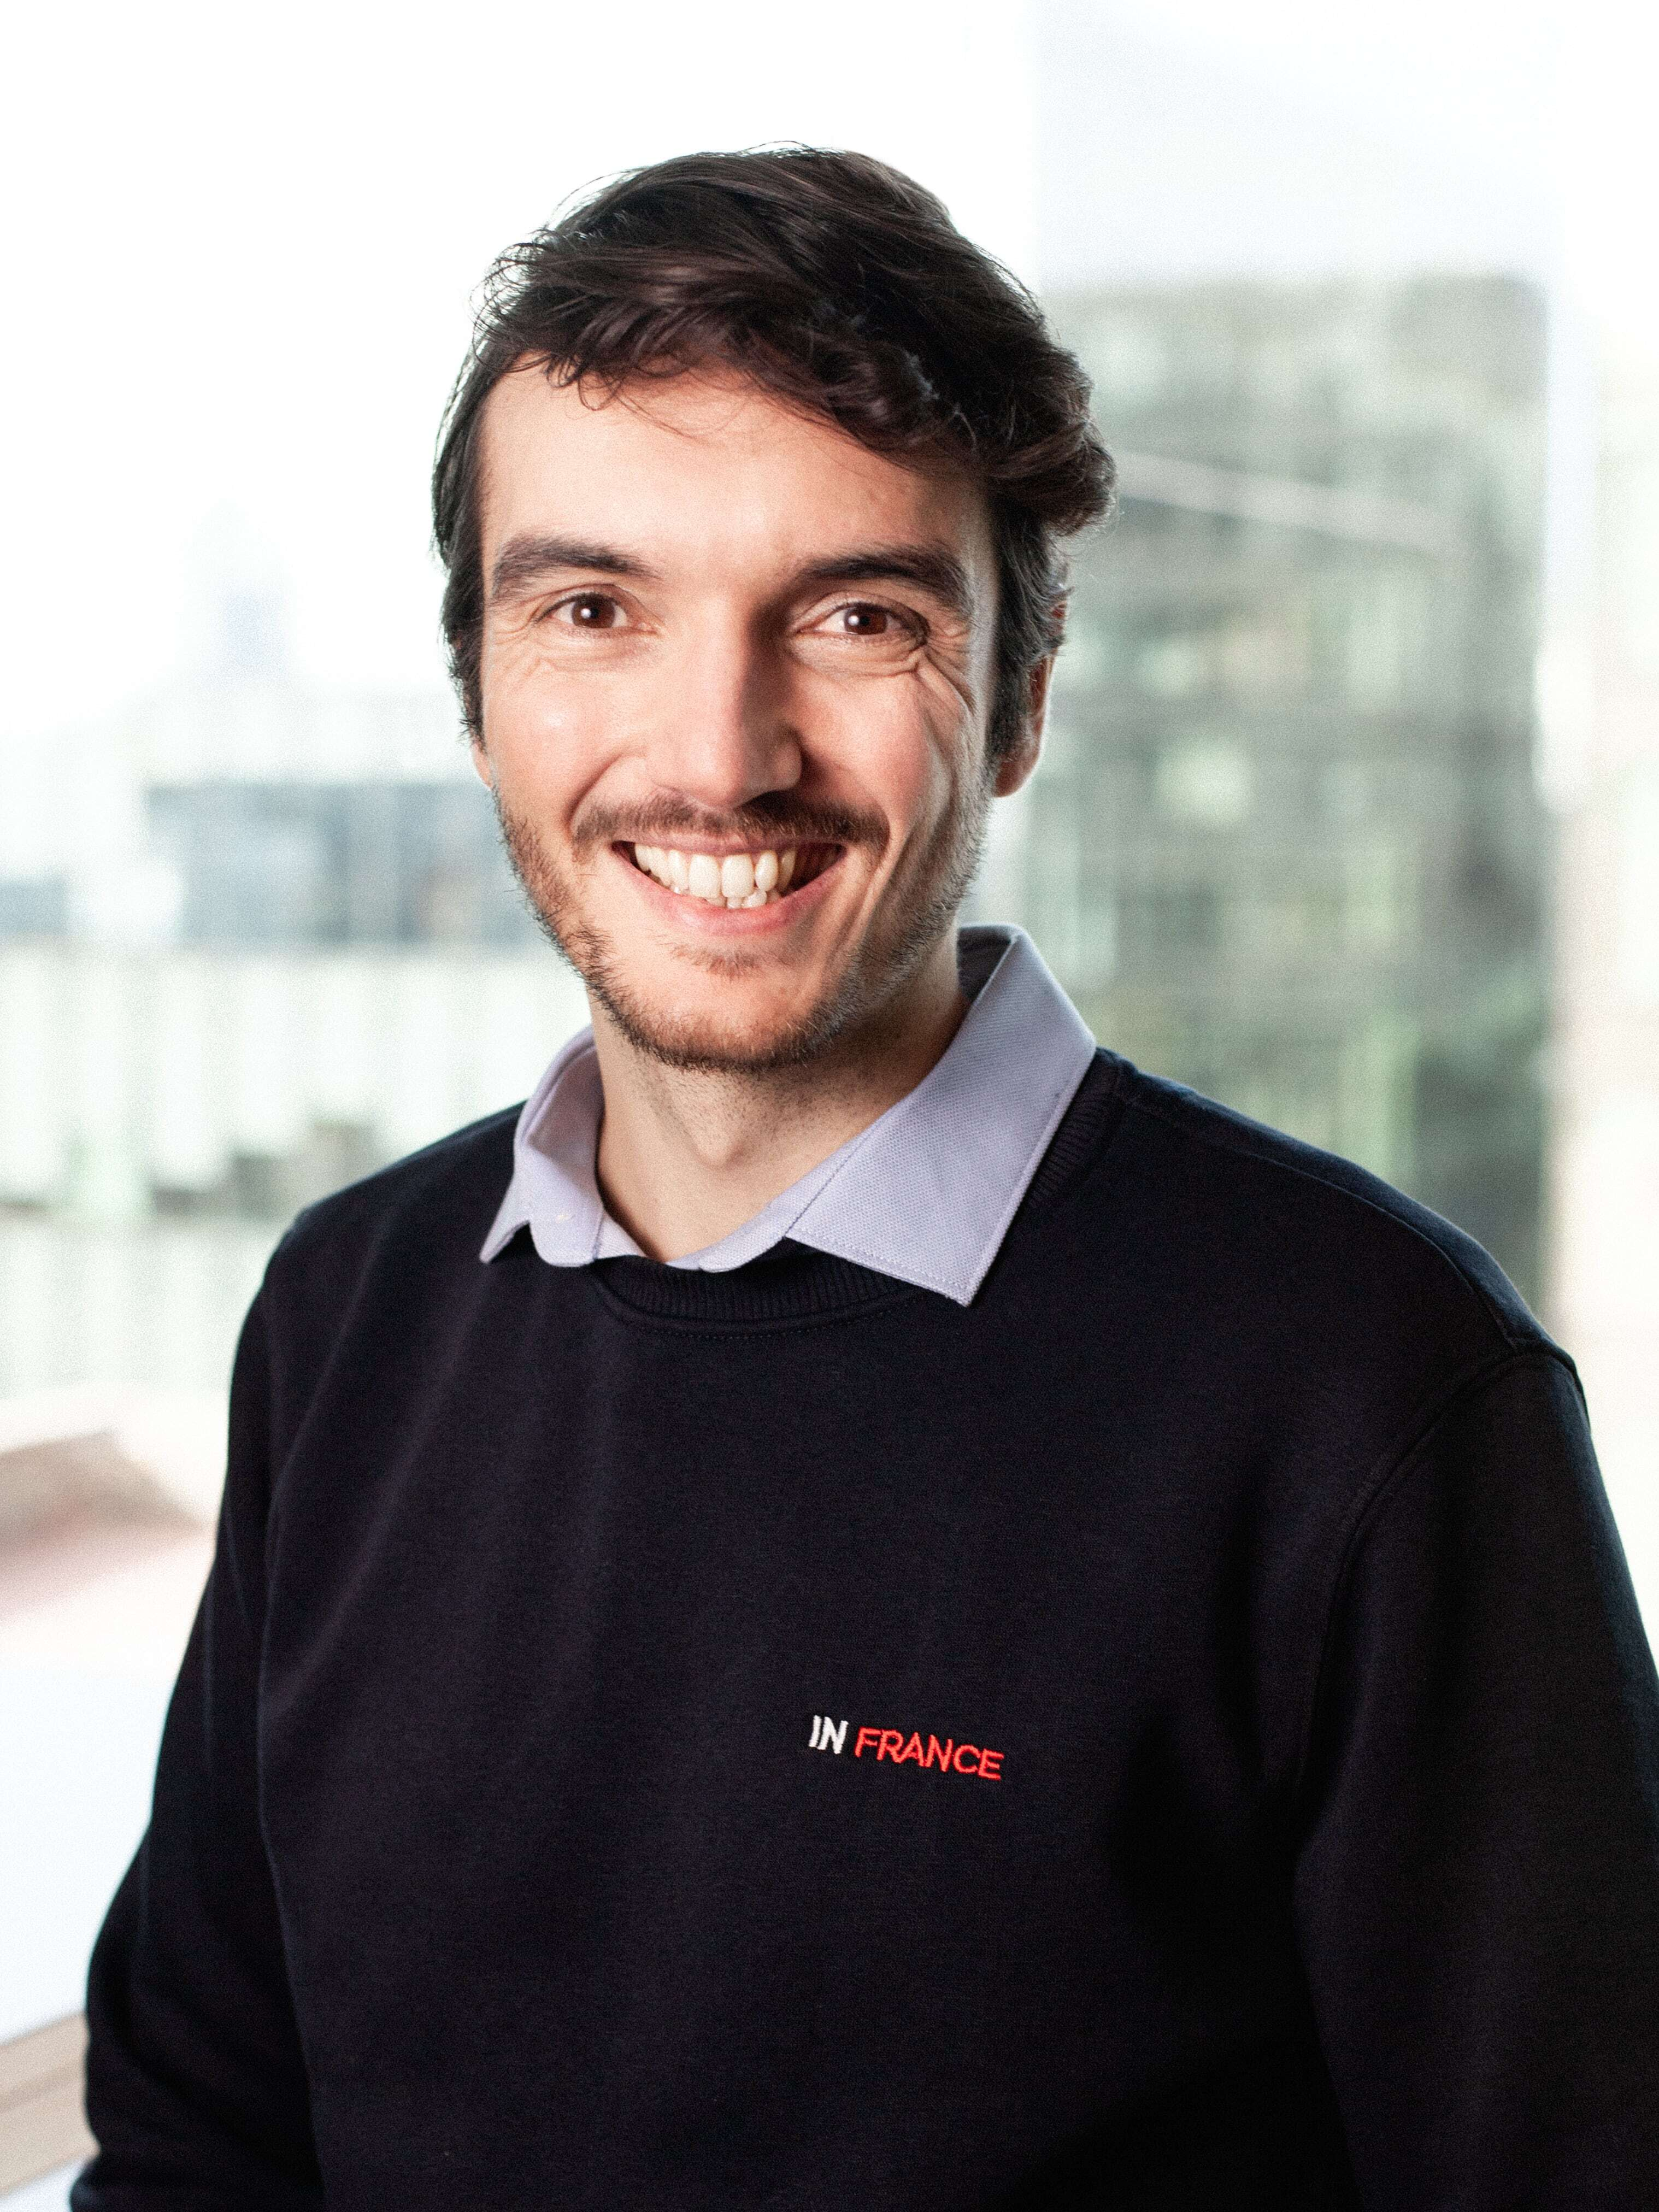
\includegraphics[width=5cm]{image/trombine-christophe}
        \end{columns}
    \end{frame}


    \section{Les impacts}\label{sec:les-impacts}

    \subsection{Impact financier direct}\label{subsec:impact-financier-direct}
    \begin{frame}{Impact financier direct}{Réglementaire\footnote{Sanctions et mesures correctrices~: la CNIL présente le bilan 2023 de son action répressive ~: \url{https://www.cnil.fr/fr/sanctions-et-mesures-correctrices-la-cnil-presente-le-bilan-2023-de-son-action-repressive}}}
        \centering
        
\includegraphics[width=11cm]{image/sanctions-cnil-2023}
    \end{frame}

    \begin{frame}{Impact financier direct}{Détournement de moyens monétiques}
        Un backend stock directement ou indirectement des secrets comme des clés d'API (Stripe, \textit{etc}), des données financières sensibles.
        \begin{itemize}
            \item Hack de Stripe~: 70 k\$ détournés à une web designeuse\footnote{My Stripe Account Was Hacked and Stripe Said I Have To Repay \$70K, \url{https://webdesigneracademy.com/my-stripe-account-was-hacked-and-stripe-said-i-have-to-repay-70k/}}.
            \item Vol de coordonnées de cartes de crédit dans un plugin Prestashop payant \footnote{Facebook PrestaShop module exploited to steal credit cards, \url{https://www.bleepingcomputer.com/news/security/facebook-prestashop-module-exploited-to-steal-credit-cards/}}.
        \end{itemize}
    \end{frame}

    \subsection{Le risque réputationnel}\label{subsec:risque-reputationnel}
    \begin{frame}{Risque réputationnel}{La rigueur s'impose dans certains domaines}
        \textit{Normalement} un acteur sensible (finance, défense, santé) du numérique qui voit ses données fuirent, devrait disparaître\ldots
        \begin{itemize}
            \item Flow Bank~: Flow bank victime de vol de données, le régulateur ferme la banque moins d'un an plus tard\footnote{Des hackers ont accédé aux données client d’une banque en ligne, \url{https://www.20min.ch/fr/story/des-hackers-ont-accede-aux-donnees-client-dune-banque-en-ligne-736748131987}}\footnotestep\footnote{Faillite d’une banque suisse~: Entre fraude et dissimulation, découvrez les révélations chocs~!, \url{https://moneyradar.org/articles-economie-societe/fin-de-flowbank-entre-fraude-dissimulation-et-faillite-decouvrez-les-revelations-chocs/}}.
            \item Crédit Suisse~: Crédit Suisse, qui blanchit l'argent du traffic de drogue et disparaît un an plus tard\footnote{Data Leak Shows Credit Suisse’s Criminal Clientele, Bank Denies Wrongdoings, \url{https://www.financemagnates.com/institutional-forex/data-leak-shows-credit-suisses-criminal-clientele-bank-denies-wrongdoings/}}.
        \end{itemize}
    \end{frame}


    \section{Les vecteurs d'attaque}\label{sec:les-vecteurs-dattaque}

    \subsection{Le buffer overflow}\label{subsec:les-buffer-overflow}

    \begin{frame}{Buffer Overflow}{Définition}
        \begin{footnotesize}
            Le débordement de tampon désigne une anomalie qui se produit lorsqu'un logiciel écrit des données dans une mémoire tampon jusqu'à surcharger la capacité de cette dernière, entraînant ainsi l'écrasement des emplacements de mémoire adjacents.

            En d'autres termes, un trop grand nombre d'informations sont transmises dans un conteneur ne disposant pas de suffisamment d'espace et ces dernières finissent par remplacer les données situées dans les conteneurs adjacents.
            \begin{columns}
                \begin{column}{0.7\textwidth}
                    Les pirates peuvent tirer parti du débordement de tampon pour modifier la mémoire d'un ordinateur afin de perturber l'exécution d'un programme ou d'en prendre le contrôle\footnotemark.
                    \bigbreak
                    Aux États-Unis, le sujet est pris en main par la Maison Blanche qui donne chaque année ses recommandations sur la gestion de la mémoire dans le développement logiciel\footnotemark.
                \end{column}
                \begin{column}{0.3\textwidth}
                    
\includegraphics[width=3cm]{image/old-senile-at-white-house}
                \end{column}
            \end{columns}
            \footnotetext{Statements of Support for Software Measurability and Memory Safety, \url{https://www.whitehouse.gov/oncd/briefing-room/2024/02/26/memory-safety-statements-of-support/}}
            \footnotetext{Qu'est-ce que le débordement de tampon (buffer overflow)~?, \url{https://www.cloudflare.com/fr-fr/learning/security/threats/buffer-overflow/}}
        \end{footnotesize}
    \end{frame}

    \begin{frame}[fragile]{Buffer Overflow}{Example de Stack-Based Buffer Overflow\footnote{\label{hacking}Hacking, The art of exploitation, Jon Erickson, 2\textsuperscript{nd} edition}}
        Le programme \lstinline{auth-overflow.c} est un programme en C qui vérifie un mot de passe et est vulnérable à un buffer overflow~:
        % C listing
        \begin{lstlisting}[language=C,basicstyle=\tiny\ttfamily]
#include <stdio.h>
#include <stdlib.h>
#include <string.h>
int check_authentication(char *password) {
    char password_buffer[16];
    int auth_flag = 0;
    strcpy(password_buffer, password); // Not so safe at all
    if (strcmp(password_buffer, "brillig") == 0)
        auth_flag = 1;
    if (strcmp(password_buffer, "outgrabe") == 0)
        auth_flag = 1;
    return auth_flag;
}
int main(int argc, char *argv[]) {
    if (argc < 2) {
        printf("Usage: %s <password>\n", argv[0]);
        exit(0);
    }
    if (check_authentication(argv[1])) {
        printf("Access Granted.\n");
    } else {
        printf("Access Denied.\n");
    }
}
        \end{lstlisting}
    \end{frame}

    \begin{frame}[fragile]{Buffer Overflow}{Example de Stack-Based Buffer Overflow\cref{hacking}}
        % C listing
        \begin{lstlisting}[language=bash]
$ gcc auth-overflow.c -o auth-overflow
$ ./auth-overflow brillig
Access Granted.
$ ./auth-overflow $(python3 -c "print('A'*2)")
Access Denied.
$ ./auth-overflow $(python3 -c "print('A'*24)")
Access Denied.
$ ./auth-overflow $(python3 -c "print('A'*25)")
*** stack smashing detected ***: terminated
Abandon (core dumped)
        \end{lstlisting}
        Expliquer ce qui se passe dans ces cas~?
        \pause
        \bigbreak
        \lstinline{stack smashing detected} veut dire que GCC a détecté un buffer overflow et fait crasher le programme de manière préventive.
        Il parle de la stack, car c'est dans cette mémoire que les variables locales sont stockées.
    \end{frame}

    \begin{frame}[fragile]{Buffer Overflow}{Example de Stack-Based Buffer Overflow\cref{hacking}}
        \begin{lstlisting}[language=bash]
$ gcc auth-overflow.c -fno-stack-protector -o auth-overflow
$ ./auth-overflow $(python3 -c "print('A'*25)")
Access Denied.
$ ./auth-overflow $(python3 -c "print('A'*266)")
Erreur de segmentation (core dumped)
$ ./auth-overflow $(python3 -c "print('A'*30)")
Access Granted.
        \end{lstlisting}
        \bigbreak
        \begin{columns}
            \begin{column}{0.6\textwidth}
                Si on désactive cette protection avec l'option \lstinline{-fno-stack-protector}.
            \end{column}
            \begin{column}{0.4\textwidth}
                
\includegraphics[width=4cm]{image/programmer-head-exploding}
            \end{column}
        \end{columns}
    \end{frame}

    \begin{frame}[fragile]{Buffer Overflow}{Example de Stack-Based Buffer Overflow: remédiation possible}
        Une approche du type defensive programming consiste à limiter la taille du buffer.
        Exemple avec \lstinline{auth-overflow-size-constraint.c}~:
        % C listing
        \begin{lstlisting}[language=C,basicstyle=\tiny\ttfamily]
#include <stdio.h>
#include <stdlib.h>
#include <string.h>

int check_authentication(char *password) {
    int buffer_size = 16;
    char password_buffer[buffer_size];
    int auth_flag = 0;
    strncpy(password_buffer, password, buffer_size); // Not so safe but better
    if (strcmp(password_buffer, "brillig") == 0)
        auth_flag = 1;
    if (strcmp(password_buffer, "outgrabe") == 0)
        auth_flag = 1;
    return auth_flag;
}
int main(int argc, char *argv[]) {
    if (argc < 2) {
        printf("Usage: %s <password>\n", argv[0]);
        exit(0);
    }
    if (check_authentication(argv[1])) {
        printf("Access Granted.\n");
    } else {
        printf("Access Denied.\n");
    }
}
        \end{lstlisting}
    \end{frame}

    \begin{frame}[fragile]{Buffer Overflow}{Example de Stack-Based Buffer Overflow: remédiation possible}
        % C listing
        \begin{lstlisting}[language=bash]
$ gcc auth-overflow-size-constraint.c -o auth-overflow-size-constraint
$ ./auth-overflow-size-constraint $(python3 -c "print('A'*30)")
Access Denied.
$ ./auth-overflow-size-constraint $(python3 -c "print('A'*300)")
Access Denied.
$ ./auth-overflow-size-constraint "brillig"
Access Granted.
        \end{lstlisting}
        Expliquer ce qui se passe dans ces cas~?
        \pause
        \bigbreak
        Contrairement à \lstinline{strcpy}, \lstinline{strncpy} \textit{Copy no more than N characters of SRC to DEST}~.
        \bigbreak
        On peut en plus isoler dans un Docker ou un chroot, en cas de RCE, elle sera isolée.
    \end{frame}

    \begin{frame}{Buffer Overflow}{Exercices}
        Les exercices sont notés pour ceux qui passent y répondre au tableau.
        \bigbreak
        Exercice \execcounterdispinc{}~:
        Étudier les guidelines de la Maison Blanche sur la gestion de la mémoire dans le développement logiciel.
        \bigbreak
        Comprendre et lister ce qui est déconseillé et ce qui conseillé et pourquoi.
        Exercice \execcounterdispinc{}~:
        Comment Java prévient les buffers overflow~?
        \bigbreak
        Exercice \execcounterdispinc{}~:
        Comment Rust prévient les buffers overflow~?
    \end{frame}

    \begin{frame}{Buffer Overflow}{Ghidra}
        La décompilation/désassemblage d'un binaire est toujours possible.
        Elle peut se faire en assembleur ou dans un langage plus haut niveau comme C.
        \bigbreak
        Ghidra \textit{A software reverse engineering (SRE) suite of tools developed by NSA's Research Directorate in support of the Cybersecurity mission}\footnote{Ghidra, \url{https://ghidra-sre.org/}} permet de décompiler un C.
        C'est un framework très populaire en reverse engineering depuis sa libération 2019.
        Il vient faire de l'ombre à IDA, un software propriétaire, leader avant l'arrivée de Ghidra.
        \bigbreak
        \centering
        
\includegraphics[width=4cm]{image/GHIDRA}
    \end{frame}

    \begin{frame}{Buffer Overflow}{Ghidra}
        Ces frameworks peuvent être utilisés pour trouver des vulnérabilités du type buffer overflow dans votre stack, vos programmes, par des experts en cybersécurité dûment mandatés ou des personnes malveillantes.
        \bigbreak
        Exercice \execcounterdispinc{}~:
        \begin{itemize}
            \item Installer Ghidra.
            \item Lancer Ghidra et ouvrir les binaires \href{https://github.com/St-Michel-IT/data-security/blob/main/mystery-bin-1}{mystery-bin-1} et \href{https://github.com/St-Michel-IT/data-security/blob/main/mystery-bin-2}{mystery-bin-2}.
            Ces binaires sont issus de codes similaires à ceux vus précédemment vérifiant les mots de passe.
            \item Comparer les 2 sources, en vous basant sur le mécanisme de protection contre les buffer overflow vu précédemment, trouver lequel est vulnérable et lequel ne l'est pas.
            \item Déposer un rapport sur Teams expliquant quel binaire est vulnérable et pourquoi, lequel est safe.
            Avec les morceaux de code qui vont font dire cela et des captures d'écran.
        \end{itemize}
    \end{frame}

    \subsection{Supply chain attack}\label{subsec:supply-chain-attack}
    \begin{frame}{Supply chain attack}{Définition\footnote{Attaques de la chaîne d’approvisionnement~: Exemples et contre-mesures, \url{https://www.fortinet.com/fr/resources/cyberglossary/supply-chain-attacks}}}
        Attaque de la chaîne d'approvisionnement en français.
        \bigbreak
        Une attaque de la chaîne d’approvisionnement fait référence au fait que quelqu’un utilise un fournisseur ou un partenaire externe qui a accès à vos données et systèmes pour infiltrer votre infrastructure numérique.
        Étant donné que la partie extérieure a obtenu le droit d’utiliser et de manipuler des zones de votre réseau, vos applications ou des données sensibles, l’attaquant doit uniquement pénétrer dans les défenses du tiers ou programmer une faille dans une solution proposée par un fournisseur pour infiltrer votre système.
        \bigbreak
        Possible entre logiciels propriétaires et logiciels open source.
        Mais plus connu dans l'open source, qui peut par la suite aller dans le propriétaire.
    \end{frame}

    \begin{frame}{Supply chain attack}{Comparaison des écosystèmes\footnote{\label{snyk}The state of open source security report, \url{https://res.cloudinary.com/snyk/image/upload/v1551172581/The-State-Of-Open-Source-Security-Report-2019-Snyk.pdf}}}
        \centering
        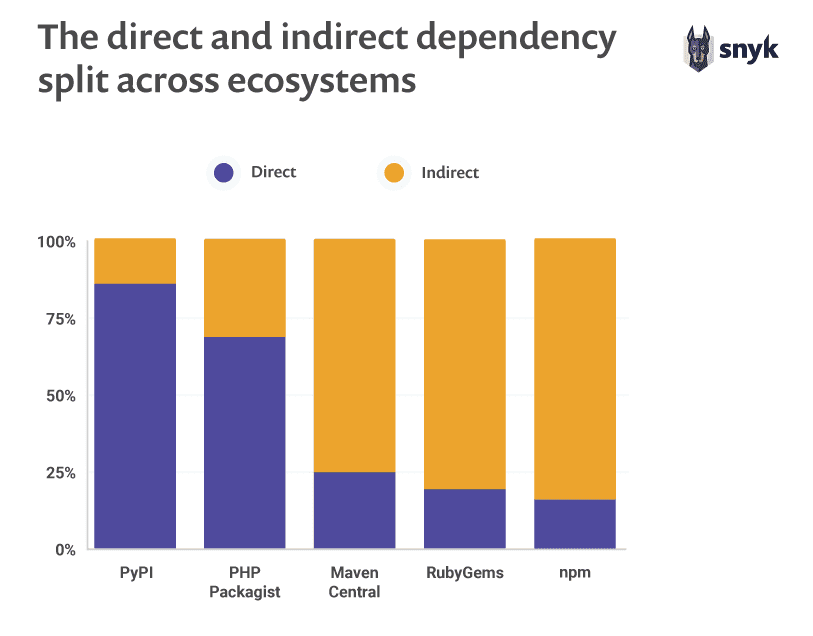
\includegraphics[width=9cm]{image/vuln-direct-indirect-dependencies}
    \end{frame}

    \begin{frame}{Supply chain attack}{Comparaison des écosystèmes\cref{snyk}}
        \centering
        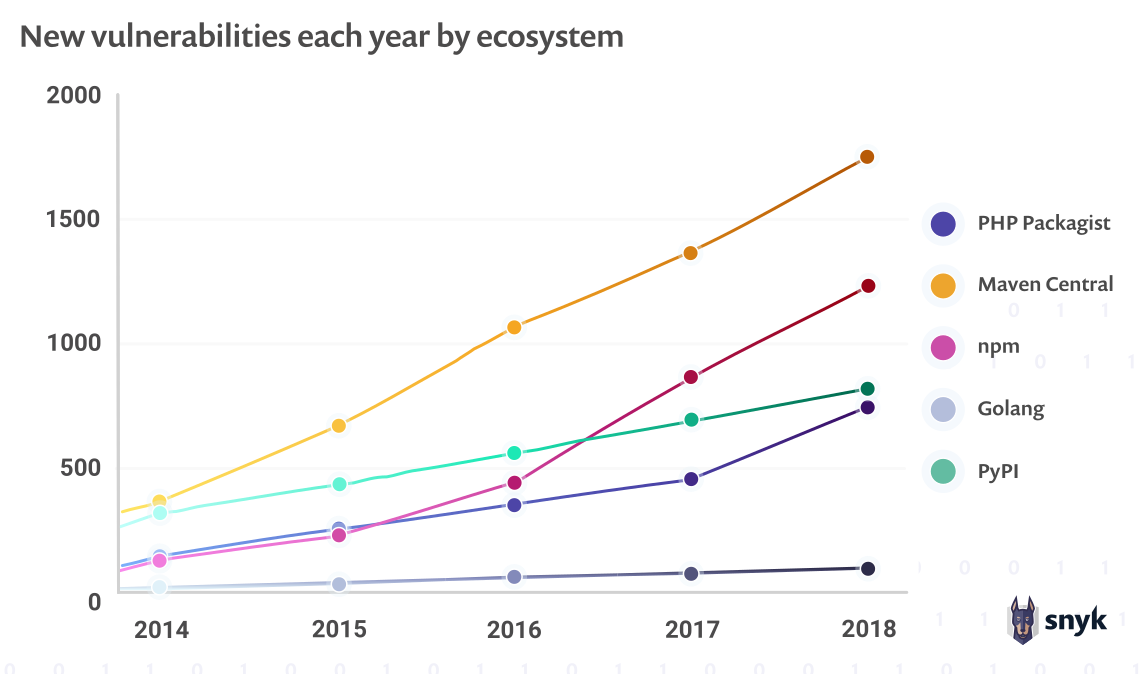
\includegraphics[width=9cm]{image/vuln-created}
    \end{frame}

    \begin{frame}{Supply chain attack}{Vulnérabilités ignorées par les écosystèmes\footnote{\label{snyk2023}2023 State of Open Source Security Report 2019, \url{https://go.snyk.io/state-of-open-source-security-report-2023-dwn-typ.html}}}
        \centering
        \begin{columns}
            \column{0.4\textwidth}
            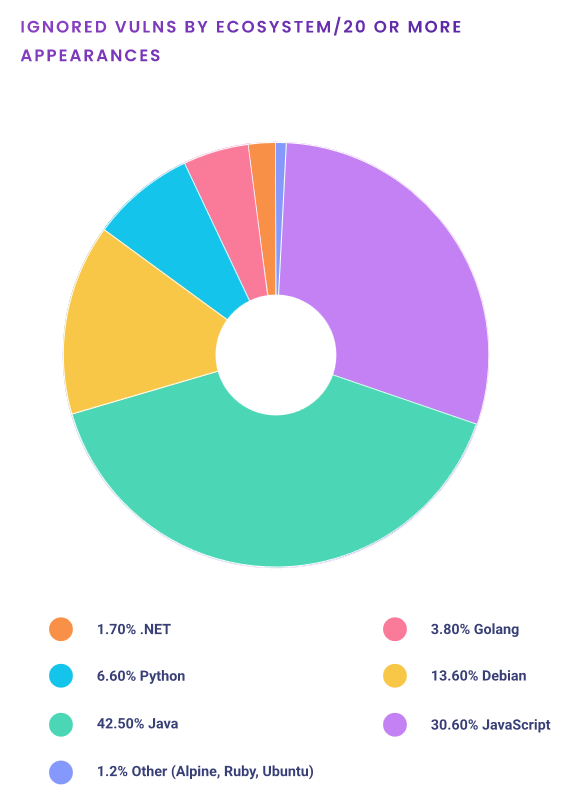
\includegraphics[width=4cm]{image/vuln-by-ecosystem}
            \column{0.6\textwidth}
            JavaScript et Java sont toujours les bons derniers en 2023\ldots
        \end{columns}
    \end{frame}

    \begin{frame}{Supply chain attack}{Remédiations~: Ne pas \textquote{tirer} n'importe quelle dépendance}
        Les usages de certains packages NPM posent questions~:
        \begin{itemize}
            \item \href{https://www.npmjs.com/package/is-number}{\lstinline{is-number}}~: 69 M téléchargements par semaine.
            \item \href{https://www.npmjs.com/package/is-odd}{\lstinline{is-odd}}~: 290 K téléchargements par semaine.
            \item \href{https://www.npmjs.com/package/is-even}{\lstinline{is-even}}~: 131 K téléchargements par semaine.
        \end{itemize}
        A-t-on vraiment besoin de ces packages~?
        \bigbreak
        \centering
        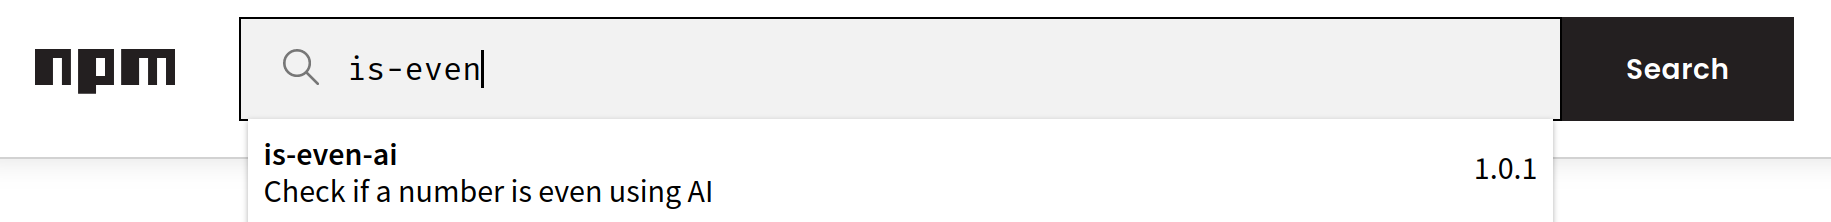
\includegraphics[width=10cm]{image/ai-everywhere}
        \flushleft
        \bigbreak
        A-t-on vraiment besoin d'IA~?
        \bigbreak
        IMHO c'est sans aucun doute un \textit{scam} \emoji{exploding-head}.
        A minima un \textit{scam} intellectuel et mathématique.
        \begin{dangercolorbox}
            Estimer le bénéfice/risque (de supply chain attack) de l'usage de ces packages.
        \end{dangercolorbox}
    \end{frame}

    \begin{frame}{Supply chain attack}{Remédiations~: Les outils de scanning\cref{snyk2023}}
        Diminution globale peut être dûe aux outils de scanning, SonarQube, CodeQL, Docker Desktop, NPM, \textit{etc}.
        \bigbreak
        \centering
        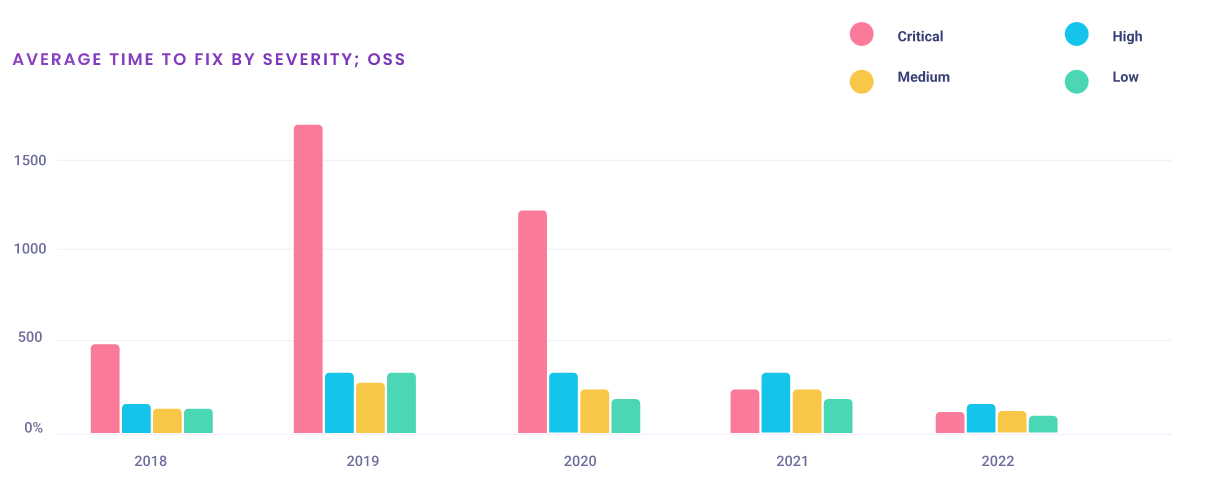
\includegraphics[width=10cm]{image/vuln-time-to-fix}
        \flushleft
        \begin{dangercolorbox}
            Lire les résultats des outils de scanning et se mettre en action.
        \end{dangercolorbox}
    \end{frame}

    \begin{frame}{Supply chain attack}{Exercice}
        Exercice \execcounterdispinc{}~:
        Vous êtes admin système et vous maintenez un pool de scripts Python qui automisent des tâches avec l'API Azure.
        \bigbreak
        Trouvez un outil qui scanne vos scripts et les dépendances de ces derniers pour détecter des vulnérabilités potentielles.

        L'outil doit présenter un rapport clair et précis des vulnérabilités détectées.
        \bigbreak
        Testez l'outil sur un script/code de votre choix et présentez le rapport.
    \end{frame}

    \subsection{Path Traversal}\label{path-traversal}


    \begin{frame}{Path Traversal}{définition\footnote{Path Traversal\url{https://owasp.org/www-community/attacks/Path_Traversal}}}
        Cette attaque vise à accéder à des fichiers et répertoires qui sont stockés en dehors du dossier racine du site web ou censés être hors des droits de l'attaquant.
        En manipulant des variables qui font références à des fichiers avec des chemins \textquote{dot-dot-slash \lstinline{../}} et ses variations ou en utilisant des chemins de fichiers absolus, il peut être possible d'accéder à des fichiers et répertoires arbitraires stockés sur le système de fichiers, y compris le code source de l'application ou des fichiers de configuration et des données sensibles.
        L'OS et ses droits ont un rôle à jouer, car l'attaquant a les droits du serveur web.
        \bigbreak
        Cette attaque est également connue sous les noms de \textquote{dot-dot-slash}, \textquote{directory traversal}, \textquote{directory climbing} et \textquote{backtracking}.
    \end{frame}

    \begin{frame}{Path Traversal}{Examples}
        Tout le monde est ou a été touché~:
        \begin{itemize}
            \item Nginx si on oublie le trailing slash dans la configuration\footnote{nginx alias misconfiguration allowing path traversal , \url{https://davidhamann.de/2022/08/14/nginx-alias-traversal/}}.
            \item Apache en 2021, Path Traversal menant à une RCE \emoji{face-screaming-in-fear}\footnote{Apache HTTP Server Path Traversal \& Remote Code Execution (CVE-2021-41773 \& CVE-2021-42013), \url{https://blog.qualys.com/vulnerabilities-threat-research/2021/10/27/apache-http-server-path-traversal-remote-code-execution-cve-2021-41773-cve-2021-42013}}.
            \item Dans \lstinline{node-static}, un serveur de fichiers statiques\footnote{Directory Traversal, \url{https://security.snyk.io/vuln/SNYK-JS-NODESTATIC-3149928}}.
            \item Many more\ldots
        \end{itemize}
    \end{frame}

    \begin{frame}{Path Traversal}{Remédiation}
        Les bonnes pratiques suivantes sont à suivre pour éviter les risques de Path Traversal~:
        \begin{itemize}
            \item Les URL doivent retourner des données sur la base de l'identifiant de l'entité et non sur la base du chemin sur le système de fichier.
            \item Mettre à jour les serveurs web et les applications pour limiter les zéros days.
            \item Utiliser des outils de scanning pour détecter les vulnérabilités.
            \item Utiliser des librairies faites pour ramener des fichiers de manière sécurisée.
            Tous les frameworks modernes ont des librairies pour cela.
            \item Isoler le serveur web dans un chroot ou un container.
        \end{itemize}
    \end{frame}

    \begin{frame}{Path Traversal}{Exercice \execcounterdispinc{}}
        Etudier la documentation du framework web Python Flask et trouver 2 méthodes qui permettent de servir des fichiers statiques de manière sécurisée.
        \bigbreak
        \centering
        
\includegraphics[width=6cm]{image/police-blocking-the-road}
    \end{frame}


    \section{La mauvaise configuration du serveur}\label{sec:configuration-serveur}

    \begin{frame}{Mauvaise configuration du serveur}{Configuration de Nginx ou Apache}
        Des données, codes source et fichiers de configuration peuvent être exposés faute d'une configuration correcte du serveur web.
        \bigbreak
        Example, quand Nginx exécute un fichier \lstinline{*.php} ce n'est pas pareil que s'il est indexé par un serveur web~!
        \bigbreak
        \begin{columns}
            \begin{column}{0.6\textwidth}
                Si on cherche avec le Google Dork \lstinline{intitle:"index of"} on trouve des répertoires indexés par des serveurs web.
                Donc avec \lstinline{intitle:"index of" wp-config.php} on trouve des fichiers de configuration de Wordpress et les identifiants de connection aux bases.

            \end{column}
            \begin{column}{0.4\textwidth}
                \centering
                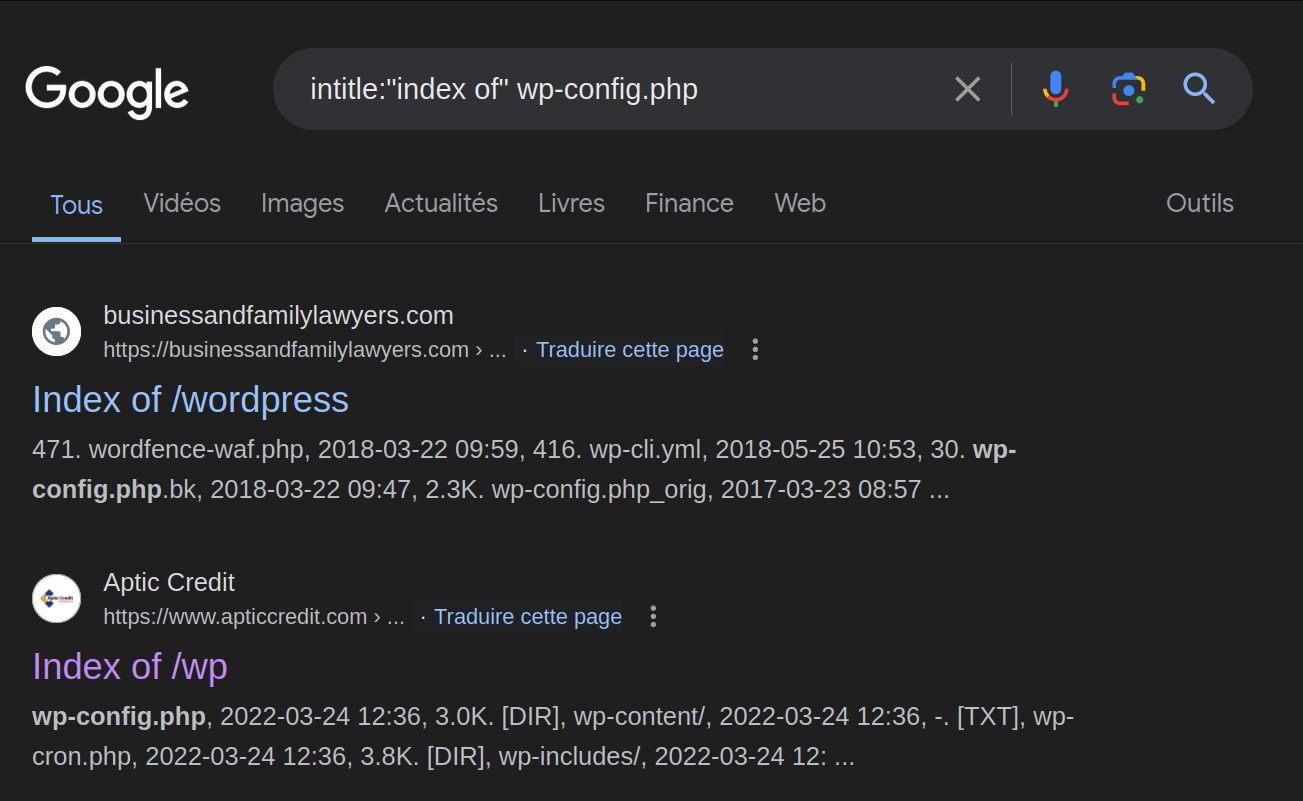
\includegraphics[width=5cm]{image/dork-on-google}
            \end{column}
        \end{columns}
    \end{frame}

    \begin{frame}{Mauvaise configuration du serveur}{Configuration de Nginx ou Apache}
        Pour ne pas indexer la configuration et le code source de votre site web, il faut ajouter les lignes suivantes dans la configuration de Nginx ou Apache~:
        \begin{itemize}
            \item Apache~: Rajouter \lstinline{Options -Indexes} dans le fichier \lstinline{.htaccess}.
            \item Nginx~: Dans le fichier de configuration, rajouter \lstinline{autoindex off;} dans la \lstinline{location}.
        \end{itemize}
        De plus un fichier \lstinline{*.php} doit être exécuté uniquement.
        \bigbreak
        \centering
        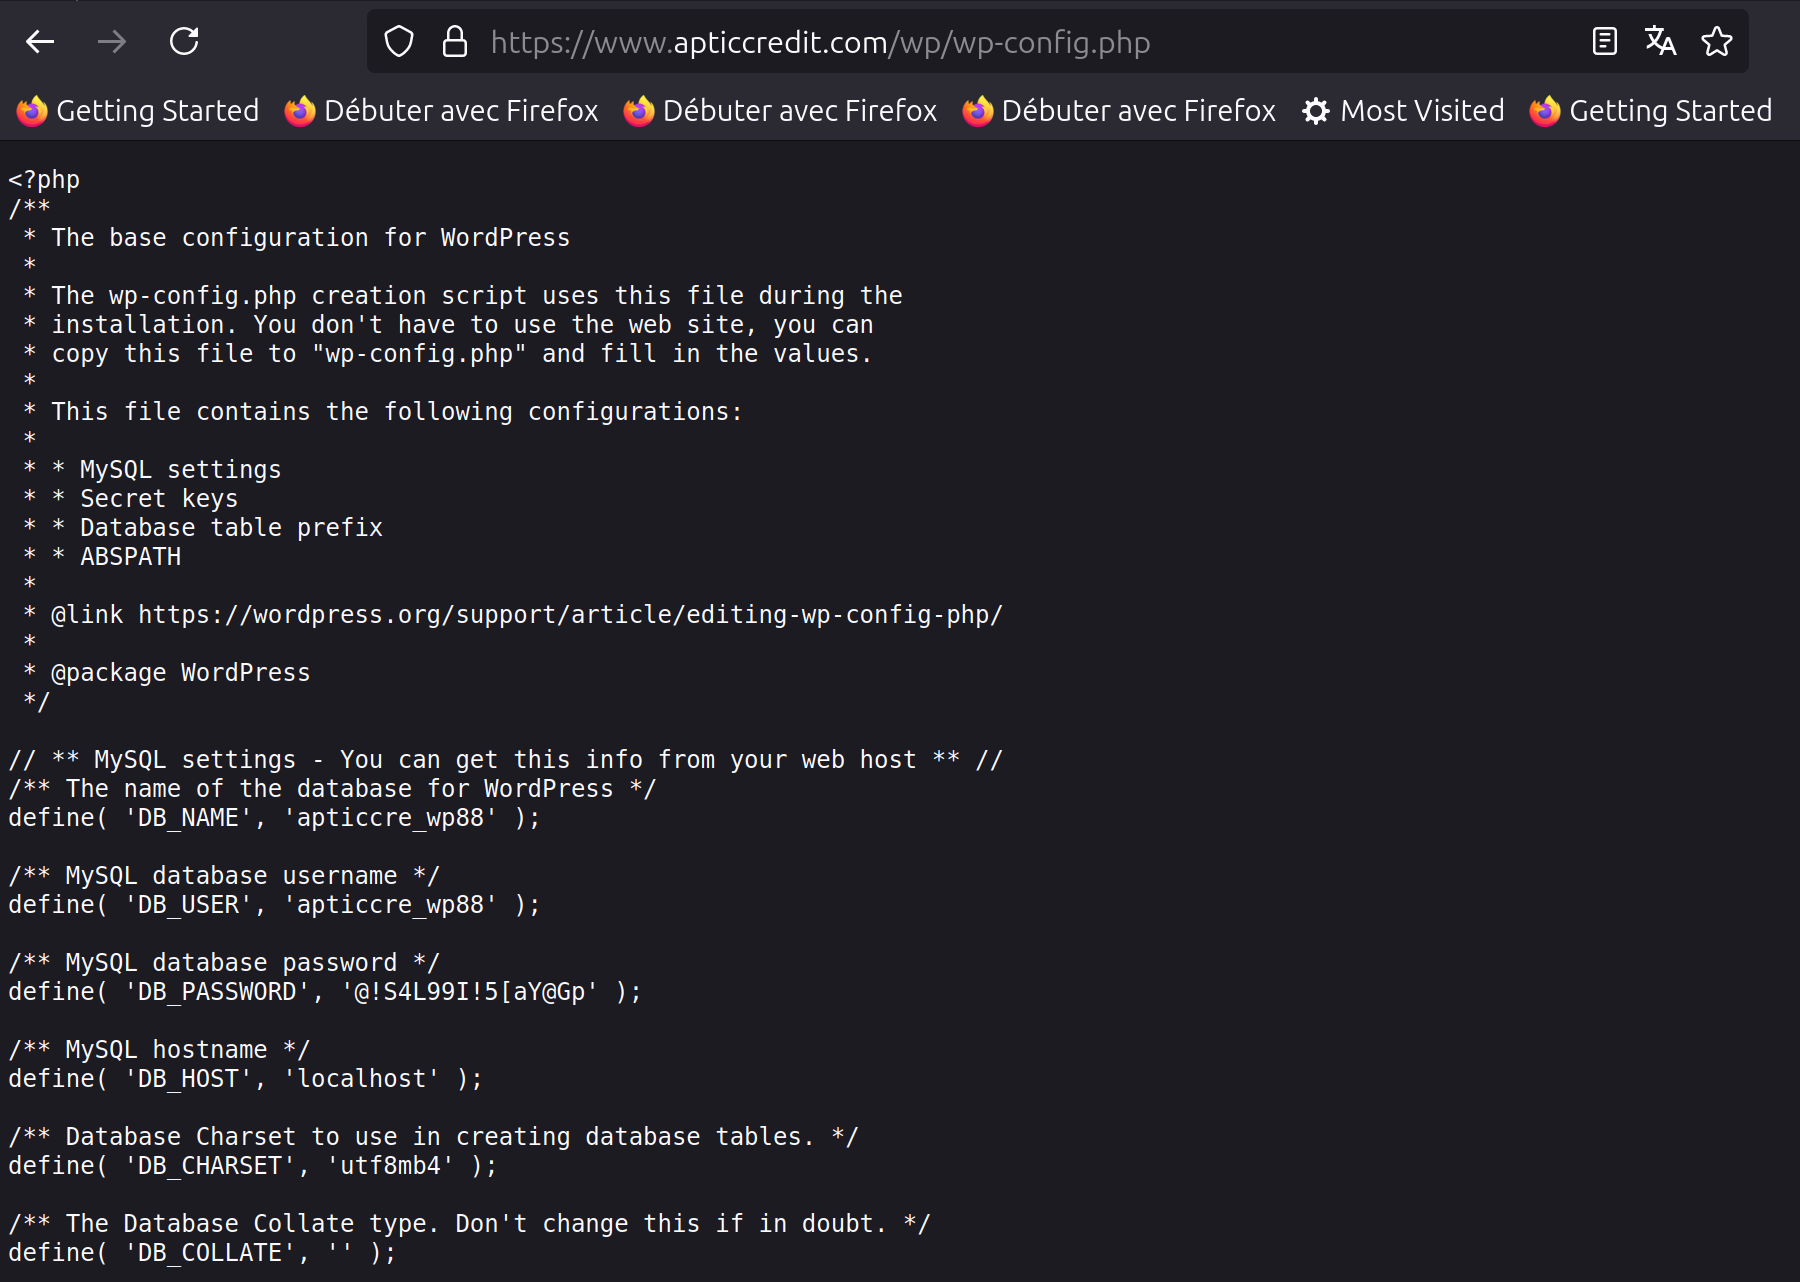
\includegraphics[width=6cm]{image/php-to-execute}
    \end{frame}

    \begin{frame}{Mauvaise configuration du serveur}{Configuration de Nginx ou Apache}
        On peut donc accéder aux données en base à partir de fichiers de configuration ou de sources.
        \bigbreak
        On peut parfois accéder \href{https://www.google.com/search?q=intitle\%3A\%22index+of+sqldump\%22}{directement aux données}~:
        \bigbreak
        \centering
        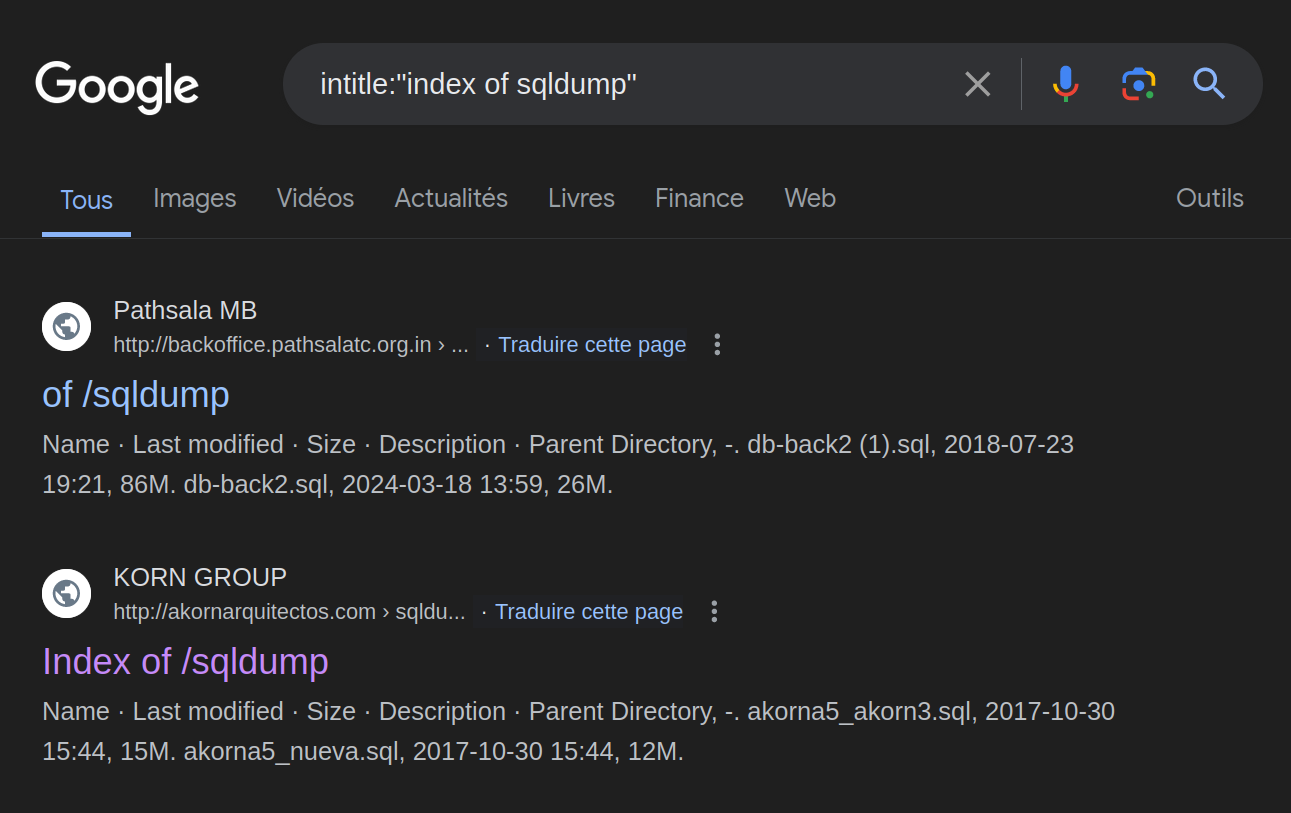
\includegraphics[width=8cm]{image/dork-sqldump}
    \end{frame}

    \begin{frame}{Mauvaise configuration du serveur}{Exercice}
        Exercice \execcounterdispinc{}~:
        Expliquer quelle(s) mauvaise(s) configuration(s) du serveur peuvent mener à la fuite de données du slide précédent.
        \bigbreak
        Exercice \execcounterdispinc{}~:
        Quels fichiers de configuration des \textquote{robots d'indexation} peuvent être utilisés pour ajouter une couche de sécurité et limiter en théorie l'indexation de fichiers sensibles~?
        Exercice \execcounterdispinc{}~:
        Quelle information sensible ne doit pas être donnée au \textquote{robots d'indexation}~?
    \end{frame}

    \begin{frame}{Mauvaise configuration du serveur}{Les fichiers de log}
        \centering
        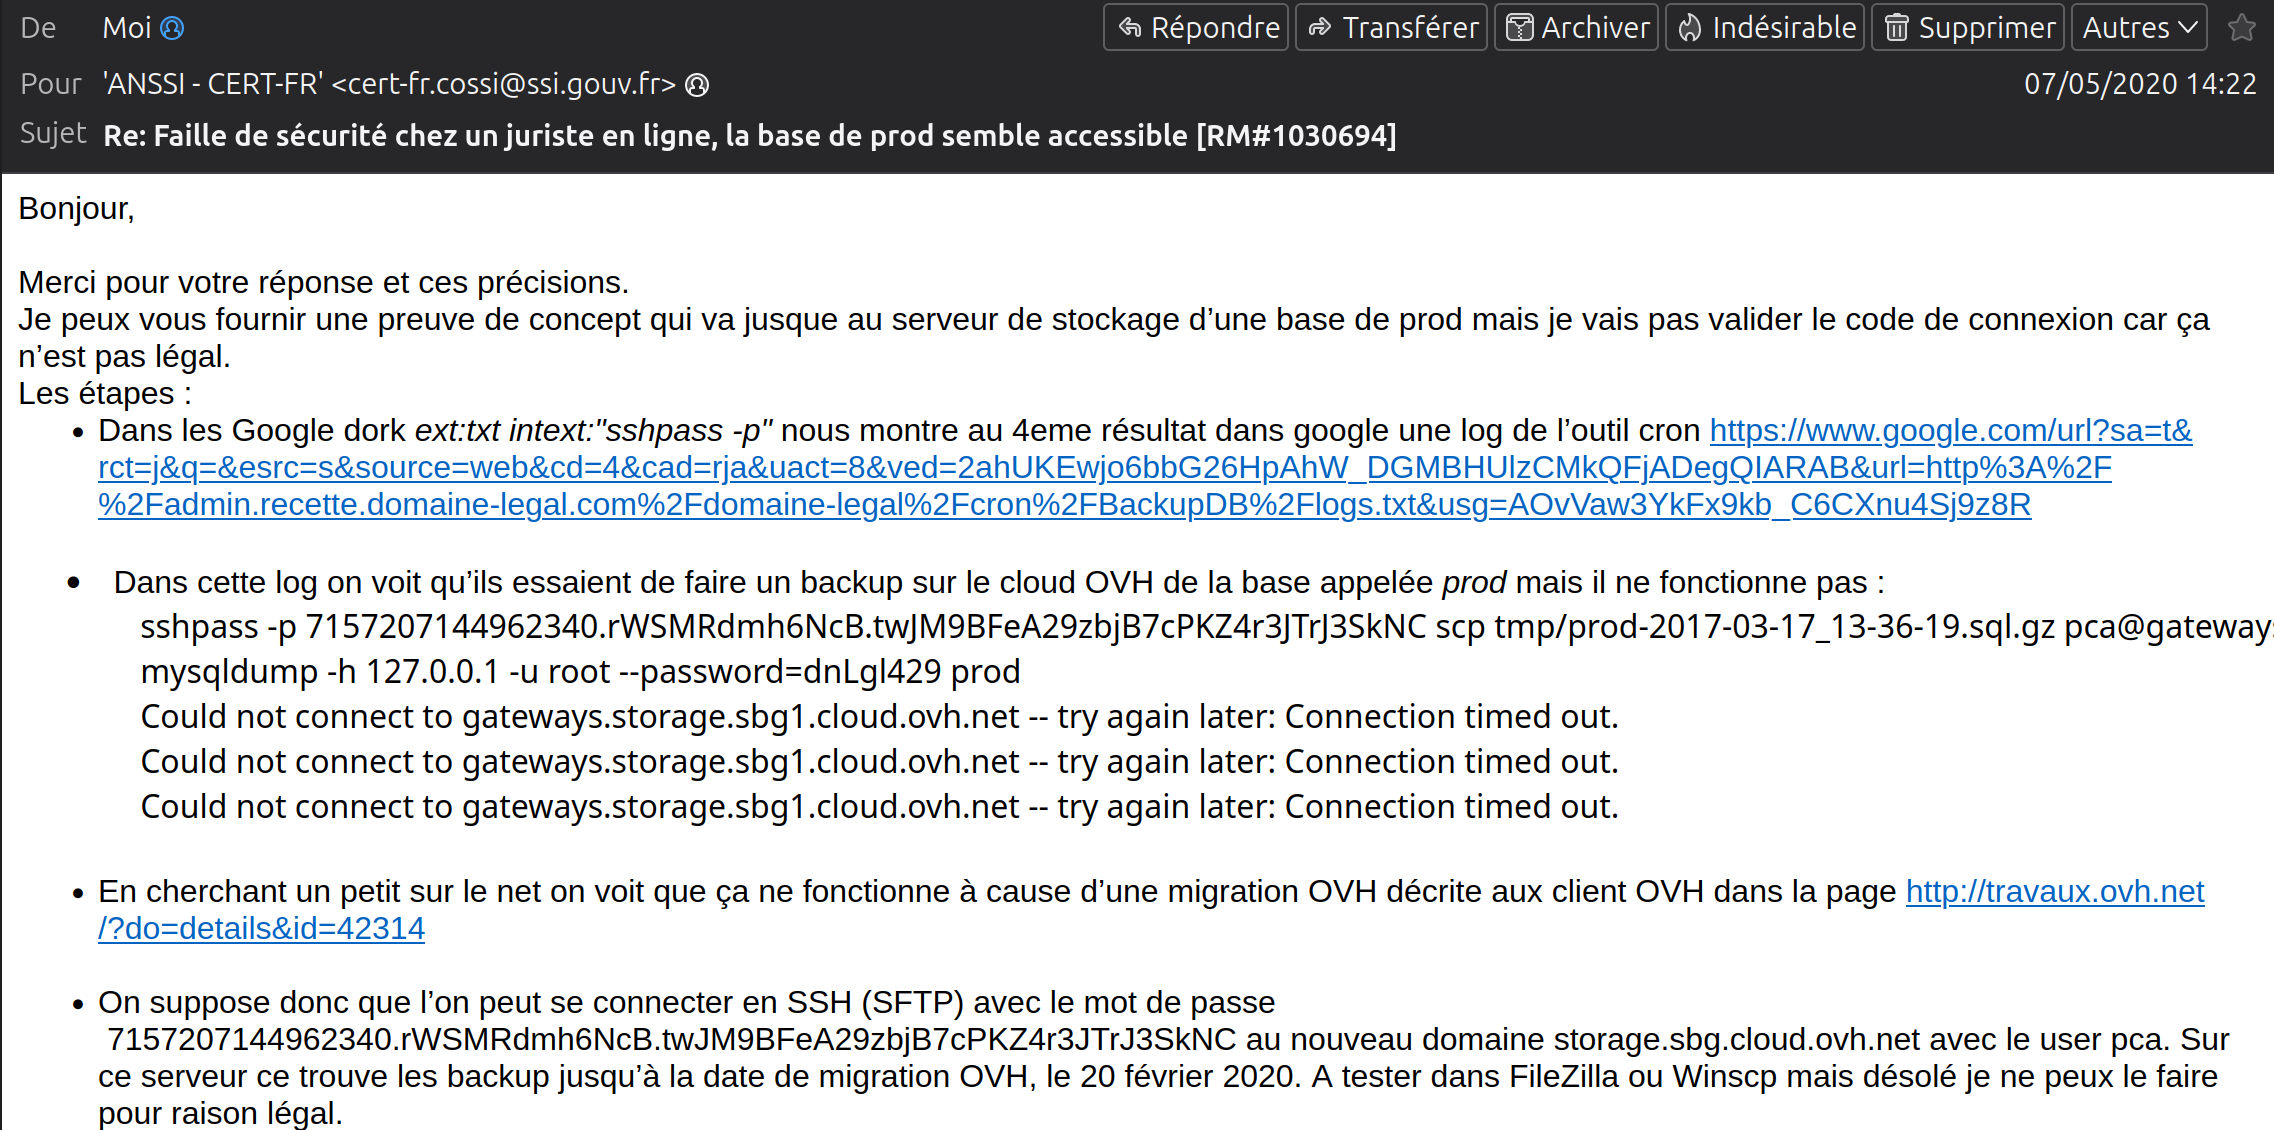
\includegraphics[width=12cm]{image/mail-anssi}
    \end{frame}


    \section{Développer le serveur applicatif}\label{sec:dev-serveur-applicatif}

    \subsection{OAuth 2}\label{subsec:oauth-2}
    \begin{frame}{OAuth2}{Définition\footnote{OAuth 2.0, \url{https://oauth.net/2/}}}
        \begin{columns}
            \begin{column}{0.6\textwidth}
                OAuth 2.0 est le protocole de référence dans l'industrie pour l'autorisation.

                Il met l'accent sur la simplicité pour les développeurs clients tout en fournissant des flux d'autorisations spécifiques pour les applications web, les applications de bureau, les téléphones mobiles et les appareils de salon.
                Cette spécification et ses extensions sont développées au sein du groupe de travail OAuth de l'IETF~.
            \end{column}
            \begin{column}{0.4\textwidth}
                \centering
                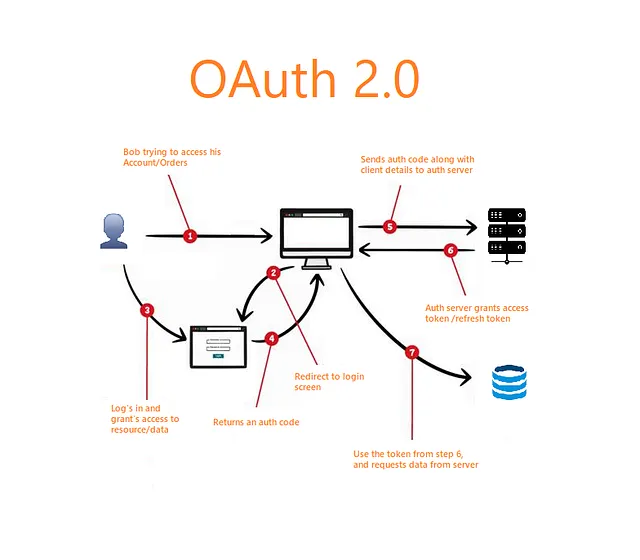
\includegraphics[width=6cm]{image/oauth2-flow}
            \end{column}
        \end{columns}
    \end{frame}

    \begin{frame}{OAuth2}{Définition\footnote{Qu'est-ce que l'OAuth~? \url{https://www.cloudflare.com/fr-fr/learning/access-management/what-is-oauth/}}}
        L'OAuth est une norme technique permettant de donner des autorisations aux utilisateurs.
        Il s'agit d'un protocole permettant de transmettre une autorisation d'un service à un autre sans partager les informations d'identification de l'utilisateur, tel qu'un nom d'utilisateur et un mot de passe.
        Avec l'OAuth, un utilisateur peut se connecter à une plateforme, puis être autorisé à effectuer des actions et à consulter des données sur une autre plateforme.
        \bigbreak
        L'OAuth permet de transmettre l'autorisation d'une application à une autre, quelle que soit la nature des deux applications.
        L'OAuth est l'une des méthodes les plus couramment utilisées pour transmettre l'autorisation d'un service d'authentification unique (SSO) à une autre application cloud, mais il peut être utilisé entre deux applications quelconques.
        L'OAuth est un des protocoles les plus utilisés.
    \end{frame}

    \begin{frame}{OAuth2}{Différence autorisation authentification}
        Exercice \execcounterdispinc{}~:
        Expliquer la différence entre l'authentification et l'autorisation.
        \bigbreak
        Exercice \execcounterdispinc{}~:
        Quels sont les avantages de l'autorisation~?
        \bigbreak
        Exercice \execcounterdispinc{}~:
        Quels sont les avantages de l'authentification~?
        En se basant sur votre compréhension de l'autorisation, qu'est que l'on ne trouvera dans un serveur OAuth2 comme \url{https://github.com/authlib/example-oauth2-server} et qu'il reste à implémenter~?
    \end{frame}

    \begin{frame}{OAuth2}{OpenID Connect ou OIDC}
        C'est une surcouche d'OAuth2 qui ajoute l'authentification.
        Elle n'a pas de point d'API pour les données de l'utilisateur, mais encode les données de l'utilisateur au format JWT~.
        Ce JWT est signé par le serveur OIDC\footnote{Oauth2 vs OpenId Connect, \url{https://www.ilex-international.com/fr/federation-identite/oauth2-vs-openid-connect}}~.

        Le JWT est signé de manière symétrique ou asymétrique, ce qui permet de vérifier son authenticité côté client.
        \bigbreak
        Le client est l'application à laquelle OAuth autorise l'accès.
    \end{frame}

    \begin{frame}{OAuth2}{L'application cliente ou client}
        Le client n'a besoin que de l'ID du client et du secret du client pour obtenir un token d'accès.
        \bigbreak
        Il doit passer au serveur une URI de redirection, parfois aussi appelée callback URL, pour recevoir le token d'accès.
        \bigbreak
        De nombreux clouds providers ont des SDK pour faciliter l'intégration d'applications à leurs serveurs OAuth2.
        \bigbreak
        Exemple de Google GCP qui propose de connecter deux types d'applications~:
        \begin{itemize}
            \item Les publiques, accessibles aux utilisateurs hors de l'organisation du compte GCP ayant un compte Google.
            \item Les internes qui sont accessibles uniquement aux utilisateurs de l'organisation du compte GCP~.
        \end{itemize}
        Des libraries clientes sont disponibles pour les langages de programmation les plus courants.
    \end{frame}

    \begin{frame}{OAuth2}{L'application cliente ou client}
        De nombreuses offres de SAAS OAuth2 sont disponibles pour les développeurs.
        Parmi elles Auth0 by Oka est un SAAS dédié aux services autour de OAuth2\footnote{Secure access for everyone But not just anyone\url{https://auth0.com/}}.
        \bigbreak
        C'est la partie serveur du protocole.
        Auth0 tente d'abstraire la complexité du protocole et l'instanciation d'un serveur OAuth2.
        Il n'y a pas de base de données à gérer.
        Tout est managé par Auth0.
        Pas d'écran ni de workflow de gestions des utilisateurs, des rôles, des organisations, \textit{etc}, à développer.
        \bigbreak
        Comme sur toutes ces plateformes un SDK est disponible pour les langages de programmation les plus courants et toutes les plateformes (M2M, Web, mobile).
        \bigbreak
        Exercice \execcounterdispinc{}~: Faites des groupes, créez un compte sur Auth0 et connecter l'application Flask \lstinline{flask-banque-dulac-iban.py} à Auth0.
    \end{frame}

    \begin{frame}{OAuth2}{Rappel sur le mécanisme de transfer de Cookie\footnote{Cookie and Session (I): The basic concept, \url{https://medium.com/@alysachan830/cookie-and-session-i-the-basic-concept-fea3d52bc8d3}}}
        \centering
        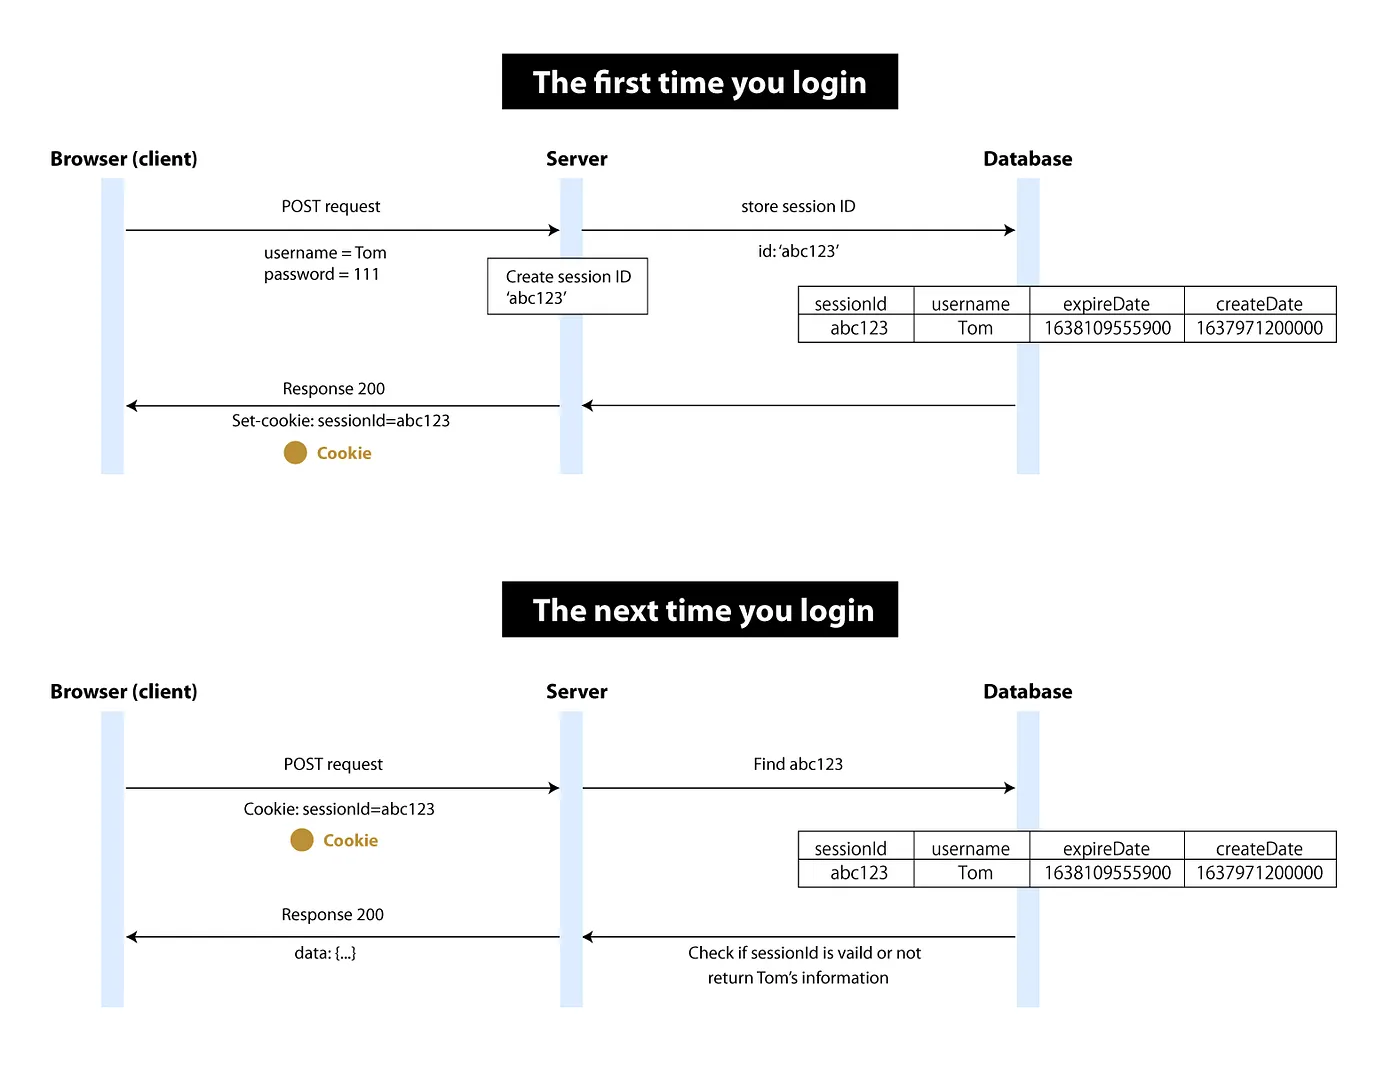
\includegraphics[width=9cm]{image/cookie-session}
    \end{frame}

    \begin{frame}{OAuth2}{Intégration d'un serveur d'autorisation}
        Exercice \execcounterdispinc{}~:
        Toujours en groupe, faites fonctionner le serveur OAuth2 comme indiqué sur \url{https://github.com/authlib/example-oauth2-server} une VM Ubuntu ou Debian d'un des clusters Proxmox.
        \bigbreak
        \centering
        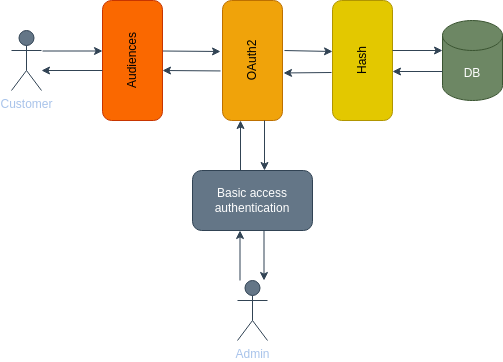
\includegraphics[width=6cm]{image/OAuth2-integration.drawio}
    \end{frame}

    \begin{frame}{OAuth2}{Intégration d'un serveur d'autorisation}
        Exercice \execcounterdispinc{}~:
        Ajouter l'algorithme de hashage de mot de passe selon les standards de sécurité modernes.
        \bigbreak
        Exercice \execcounterdispinc{}~:
        À l'aide de SQLAlchemy, créer un modèle avec tous les objets requis en base pour les données persistantes de OAuth2.
        \bigbreak
        \centering
        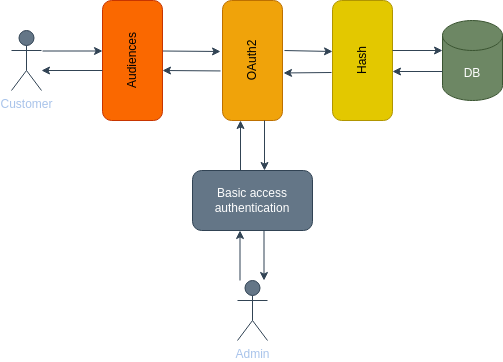
\includegraphics[width=6cm]{image/OAuth2-integration.drawio}
    \end{frame}

    \begin{frame}{OAuth2}{Intégration d'un serveur d'autorisation}
        Exercice \execcounterdispinc{}~:
        Pour administrer le SSO, créer les users, \textit{etc}.
        Une solution est de créer un compte de type super admin.
        Pour plus de simplicité, on va protéger le serveur OAuth2 avec \lstinline{auth_basic} et \lstinline{auth_basic_user_file}.
        \begin{columns}
            \begin{column}{0.6\textwidth}
                Exercice \execcounterdispinc{}~:
                Les clients à intégrer sont~:
                \begin{itemize}
                    \item \lstinline{flask-annecy-iban.py} avec JWT~.
                    \item \lstinline{flask-st-mich-iban.py} avec un appel au endpoint \lstinline{/oauth/token}~.
                \end{itemize}
                Avec le paramétrage suivant~:
                \begin{itemize}
                    \item Allowed Scope~: \lstinline{openid profile}.
                    \item Allowed Response Types~: \lstinline{code}.
                    \item Allowed Grant Types: \lstinline{authorization_code}.
                    \item Token Endpoint Auth Method~: \lstinline{client_secret_basic}.
                \end{itemize}
            \end{column}
            \begin{column}{0.4\textwidth}
                \centering
                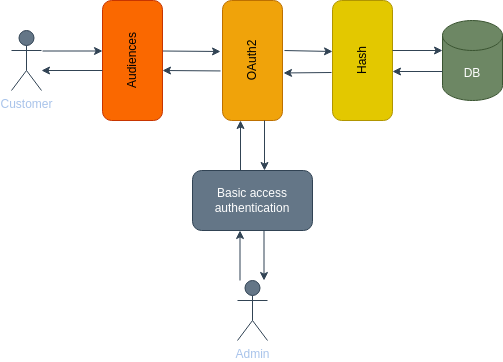
\includegraphics[width=6cm]{image/OAuth2-integration.drawio}
            \end{column}
        \end{columns}
    \end{frame}

    \begin{frame}{OAuth2}{Setup d'un serveur OAuth2 déjà développé}
        Exercice \execcounterdispinc{}~:
        Suivre le tutorial \url{https://www.ory.sh/docs/hydra/5min-tutorial} pour installer ORY Hydra avec Docker.
        \bigbreak
        Exercice \execcounterdispinc{}~:
        Suivre le tutorial \url{https://www.keycloak.org/getting-started/getting-started-docker} pour installer Keycloak et sécuriser une app via OAuth2.
    \end{frame}

    \subsection{Protection du serveur}\label{subsec:protection-serveur}
    \begin{frame}{Protection du serveur}{Sécurisation du SSH avec la cryptographie asymétrique}
        \begin{footnotesize}
            Pourquoi est-ce plus sécure d'utiliser une clé SSH plutôt qu'un mot de passe~?
            \bigbreak
            Quels algorithmes et taille de clé sont recommandés~?
            \pause
            \bigbreak
            Sur le site \url{https://jadaptive.com/ssh-key-management/the-benefits-of-ssh-key-authentication/} on trouve~:
            \begin{columns}
                \begin{column}{0.6\textwidth}
                    \begin{itemize}
                        \item Le mot de passe doit être communiqué à chaque connexion, il est donc plus vulnérable à une interception/sniffing/MITHM~.
                        La clé privée reste sur le client, elle n'est pas communiquée.
                        \item La clé SSH est plus complexe à deviner qu'un mot de passe.
                        \item On peut automatiser des taches depuis la machine cliente avec la clé SSH~.
                    \end{itemize}
                \end{column}
                \begin{column}{0.4\textwidth}
                    \centering
                    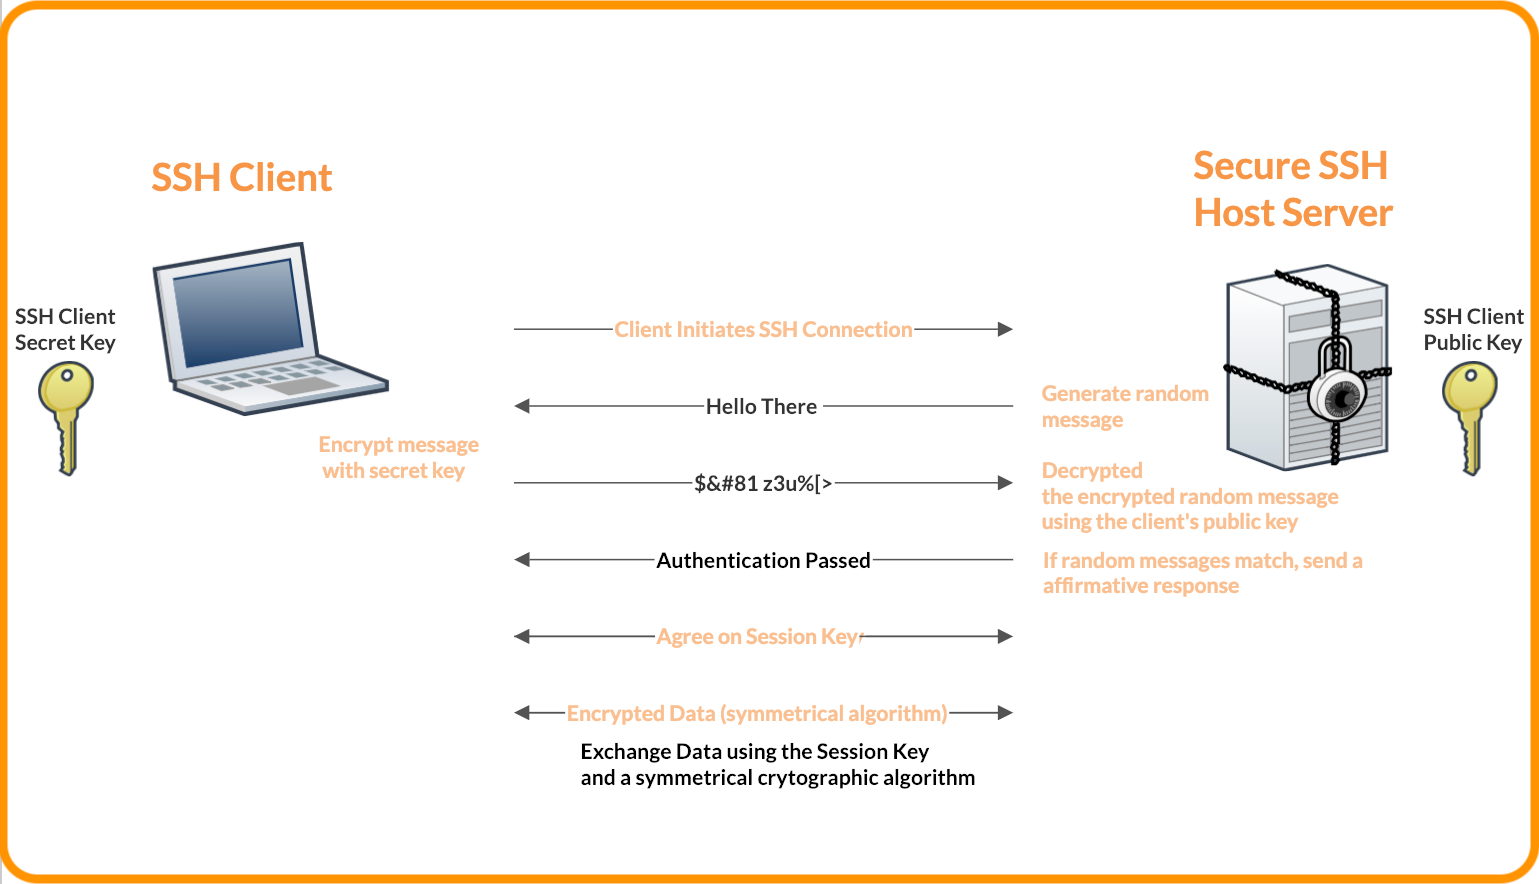
\includegraphics[width=5cm]{image/ssh-key-diagram} \\ Foxpass\footnotemark \\
                \end{column}
            \end{columns}
            \flushleft
            Exercice \execcounterdispinc{}~:
            Restreindre l'accès à la VM au SSH avec une clé SSH, aucun mot de passe.
            \footnotetext{Learn SSH Keys in Minutes, \url{https://www.foxpass.com/blog/learn-ssh-keys-in-minutes/}}
        \end{footnotesize}
    \end{frame}

    \begin{frame}{Protection du serveur}{Sécurisation des clés et des secrets}
        Que se passe-t-il si une personne malveillante a accès à votre ordinateur~?
        \bigbreak
        Par défaut, quels OS offrent quelles protections des données sur le disque~?
        \pause
        \bigbreak
        \begin{itemize}
            \item Windows~: BitLocker, n'a pas bonne réputation et dépend de l'implémentation, voir \url{https://www.youtube.com/watch?v=wTl4vEednkQ}.
            \item MacOS~: FileVault.
            \item Linux~: LUKS, \lstinline{ecryptfs-utils}, YubiKey, encryption du disque dès l'installation, \textit{etc}.
        \end{itemize}
    \end{frame}

    \begin{frame}[fragile]{Protection du serveur}{Exemple de sécurisation des clés et des secrets sous Linux}
        Par défaut, Ubuntu desktop s’installe sur une partition non
        chiffrée (encrypter, ce n’est pas français on dit chiffrer~!~).
        Tout document peut donc être lu avec un disque de
        démarrage (live CD, USB bootable, etc) ou si le disque dur
        est extrait et lu.
        \bigbreak
        Avec le package \lstinline{ecryptfs-utils} on peut chiffrer une partition~:
        \begin{lstlisting}[language=bash]
sudo apt-get install ecryptfs-utils
ecryptfs-setup-private
cp -r .ssh/ Private/ # Pour proteger les clés SSH on les déplace
ln -s /home/<mon user Ubuntu>/Private/.ssh/ . # Lien symbolique
        \end{lstlisting}
        Output~:
        \begin{lstlisting}
$ ls ~/.ssh -d -lha
lrwxrwxrwx 1 chrichri chrichri 28 janv. 14 21:27 /home/chrichri/.ssh -> /home/chrichri/Private/.ssh/
        \end{lstlisting}
        Il utilise le mot de passe de la session pour chiffrer/déchiffrer.
        Si la session n'est pas ouverte, les données sont chiffrées.
    \end{frame}


    \begin{frame}{Protection de la base}{Exemple de MySQL}
        Les configurations par défaut de MySQL sont souvent inadaptées, tant sur le plan de la sécurité que de la performance.
        \bigbreak
        Quelles options peuvent être configurées pour sécuriser une base de données MySQL~?
        \pause
        \bigbreak
        Des exemples d'options de sécurisation d'une base de données MySQL sont~:
        \begin{itemize}
            \item \lstinline{skip-networking}~: Désactive les connexions TCP/IP.
            Elle limite les connexions aux clients sur l'hôte local.
            \item \lstinline{require_secure_transport}~: Qui oblige les connexions à utiliser un chiffrement SSL/TLS et l'usage de certificats ou alors d'un Unix Domain Socket.
        \end{itemize}
        C'est quoi un Unix Domain Socket~?
    \end{frame}

    \subsection{Certificat SSL}\label{subsec:certificat-ssl}
    \begin{frame}{Apache et Nginx}{Exemple de configuration avec un certificat SSL}
        Les standards modernes de sécurité web recommandent très fortement le HTTPS et l'utilisation de certificat SSL~.
        Les clients de votre application en sont demandeur aussi.
        \bigbreak
        On peut l'acheter chez une autorité (CA) de certification comme Comodo ou autre.
        Pour seulement quelques centaines ou milliers d'Euros par an \emoji{face-with-symbols-on-mouth}.
        Ou on peut utiliser Let's Encrypt qui est gratuit.
        \bigbreak
        Let's Encrypt est un projet de CA de la \textquote{Internet Security Research Group} (ISRG) qui fournit des certificats SSL gratuits.
        Il est sponsorisé par de nombreuses entreprises du numérique.

        Le moyen le plus simple de l'installer sur votre serveur, dans votre configuration Nginx ou Apache est d'utiliser \lstinline{certbot}\footnote{Certbot, \url{https://certbot.eff.org/}}.
        \bigbreak
        Qu'apporte le certificat SSL à la sécurité de votre application~?
    \end{frame}

    \begin{frame}[fragile]{Apache et Nginx}{Exemple de configuration avec un certificat SSL}
        Avec les droits root ou en sudoer, \lstinline{certbot} installe le certificat et modifie la configuration Nginx ou Apache.

        La commande suivante~:
        \begin{lstlisting}[language=bash,basicstyle=\ttfamily\tiny]
$ sudo certbot --nginx -d your_domain
        \end{lstlisting}
        Modifie la configuration comme suit~:
        \begin{lstlisting}[basicstyle=\ttfamily\tiny]
server {
    listen 443 ssl; # Managed by Certbot

    ssl on; # Managed by Certbot
    ssl_certificate     /etc/letsencrypt/live/your_domain/fullchain.pem; # Managed by Certbot
    ssl_certificate_key /etc/letsencrypt/live/your_domain/privkey.pem; # Managed by Certbot

    server_name your_domain;

    location / {
        proxy_pass http://unix:/var/run/sock-guni;
        include proxy_params;
    }
}

server {
    listen 80 default_server; # Managed by Certbot
    server_name your_domain; # Managed by Certbot
    return 301 https://$host$request_uri; # Managed by Certbot
}
        \end{lstlisting}
    \end{frame}

    \subsection{Cryptographie Asymétrique}\label{subsec:cryptographie-asymetrique}
    \begin{frame}{Cryptographie Asymétrique}{Très brève introduction\footnote{Initiation à la cryptographie, Gilles Bubertret, 3\textsuperscript{eme} édition, Vuibert}}
        Deux grandes familles de cryptographie asymétrique~:
        \begin{itemize}
            \item RSA~: Rivest, Shamir, Adleman.
            Algorithme publié en 1978.
            Basé sur la factorisation de grands nombres premiers et l'arithmétique modulaire.
            Parce qu'il y a un déséquilibre entre la facilité de multiplication et la difficulté de factorisation.
            \item ECC~: Elliptic Curve Cryptography.
            Développé par Neal Koblitz et Victor Miller et publié en 1985.
            Ces algorithmes sont recommandés par le NIST dans les années 2000.
            On utilise des courbes elliptiques pour la cryptographie dans les clés SSH, les cartes bancaires, le Bitcoin, \textit{etc}.
        \end{itemize}
        \begin{columns}
            \begin{column}{0.8\textwidth}
                À sécurité égale, la taille des clés ECC est plus petite que celle des clés RSA~.
            \end{column}
            \begin{column}{0.2\textwidth}
                \centering
                
\includegraphics[width=2cm]{image/girl-hiding-a-secret}
            \end{column}
        \end{columns}
    \end{frame}

    \subsection{Post-quantum cryptography}\label{subsec:pqc}
    \begin{frame}{Post-quantum cryptography}{Définition\footnote{Quantum-safe Cryptography Algorithms, \url{https://research.ibm.com/projects/quantum-safe-cryptography}}}
        Concerne la conception et la mise en œuvre de protocoles qui sont censés être sécurisés contre les capacités de calcul accrues des ordinateurs quantiques.
        Les deux familles quantiques qui posent des problèmes à la cryptographie actuelle sont l'algorithme de Grover et l'algorithme de Shor.
        \bigbreak
        Grover affecte principalement la sécurité des primitives à clé symétrique (par exemple, AES, SHA-256, etc.) et la protection contre celui-ci nécessite généralement de simplement doubler la taille de la clé.
        \bigbreak
        Shor, quant à lui, est plus problématique pour la sécurité de certaines primitives à clé publique (par exemple, RSA, EC-DSA, etc.).
        Pour résister à l'algorithme de Shor, les tailles de clé devraient augmenter de manière exponentielle, ce qui les rendrait pratiquement inutilisables.
    \end{frame}

    \begin{frame}{Post-quantum cryptography}{La vidéo}
        Sur le channel Youtube \textquote{IBM Technology}, un super channel~! \url{https://www.youtube.com/watch?v=ecvCfTPRBrI}
        \bigbreak
        \centering
        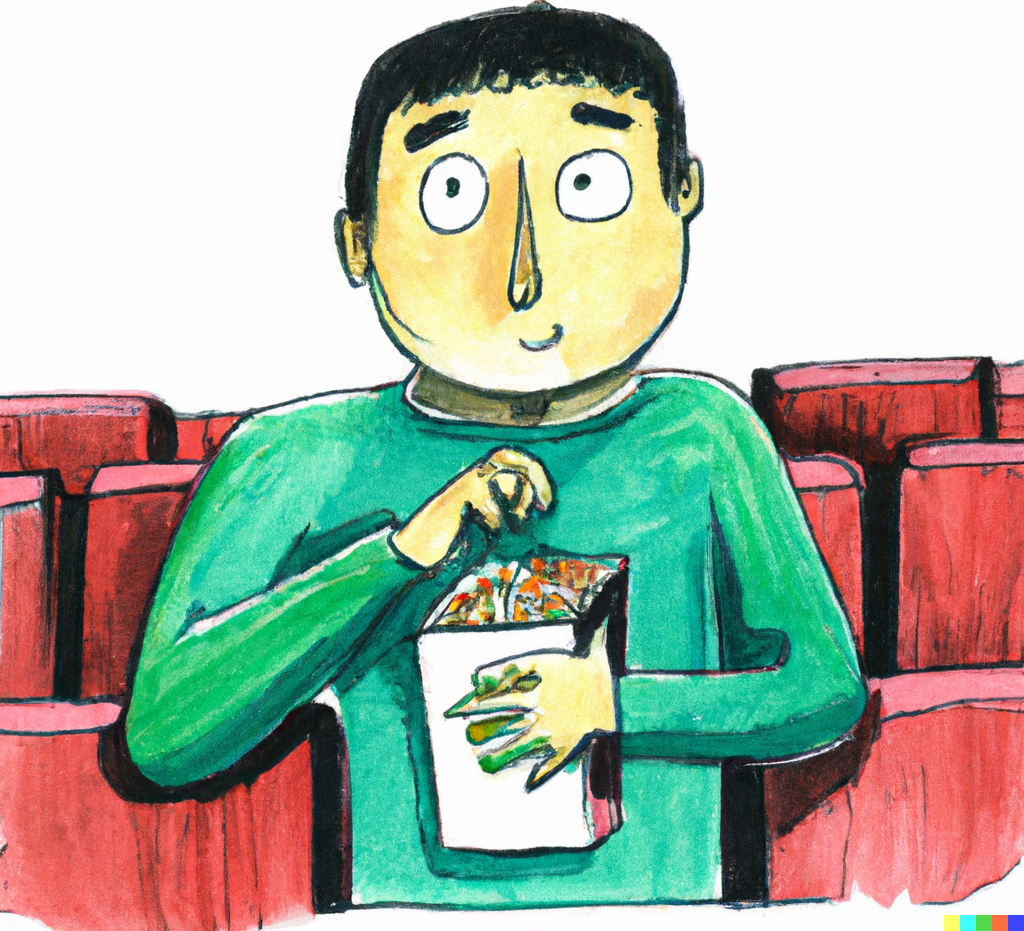
\includegraphics[width=7cm]{image/man-at-the-cinema-eating pop-corn}
    \end{frame}

    \begin{frame}{Post-quantum cryptography}{Les débuts}
        \begin{footnotesize}
            Le NIST a lancé un processus de standardisation pour les algorithmes de chiffrement post-quantique (PQC) en 2016.
            Les premiers ont été publiés en 2022.
            Parmi eux, les plus connus, voir prometteurs sont Kyber (clé publique) et Dilithium (signature), poussés en grande partie par IBM, sont deux exemples d'algorithmes de chiffrements post-quantiques basés sur les \textquote{lattice} et le \textquote{Learn With Error}.
            \bigbreak
            Cloudflare propose déjà le protocole TLS 1.3 avec l'algorithme de chiffrement post-quantique \textquote{Kyber Crystal}\footnote{\url{https://blog.cloudflare.com/post-quantum-crypto-should-be-free}}.
            \bigbreak
            L'IETF travaille sur un brouillon de la standardisation de JOSE et COSE avec Dilithium.
            Donc la PQC arrive dans OAuth2 et OpenID Connect car JOSE est utilisé pour les JWT\footnote{Post-quantum token signing with Dilithium using Duende Identity Server, \url{https://www.strathweb.com/2023/03/post-quantum-token-signing-with-dilithium-using-duende-identity-server/}}\emoji{heart}.
        \end{footnotesize}
    \end{frame}

    \begin{frame}{Cryptography}{Cryptographie avec OpenSSL\footnote{Welcome to the OpenSSL project, \url{https://github.com/openssl/openssl}}}
        \begin{itemize}
            \item \textbf{OpenSSL}~: Bibliothèque robuste et un ensemble d'outils pour l'implémentation de la cryptographie en ligne de commande et API dans divers langages.
            \item \textbf{Fonctionnalités}~:
            \begin{itemize}
                \item Chiffrement et déchiffrement.
                \item Gestion des certificats SSL/TLS.
                \item Génération de clés privées et publiques.
            \end{itemize}
            \item \textbf{Utilisation}~: Indispensable pour sécuriser les communications sur Internet, largement utilisé dans les serveurs Web.
        \end{itemize}
    \end{frame}

    \begin{frame}[fragile]{Cryptography}{Génération et utilisation d'une paire de clés RSA avec OpenSSL}
        Alice génère les clés RSA sur sa machine
        \begin{lstlisting}[language=bash,basicstyle=\ttfamily\small]
$  openssl genrsa -out cle.pem 2048
$ openssl rsa -in cle.pem -pubout -out pub.pem
writing RSA key
        \end{lstlisting}
        Sur sa machine, Bob, avec la clé publique d'Alice chiffre un secret.
        \begin{lstlisting}[language=bash,basicstyle=\ttfamily\small]
$ echo secret | openssl pkeyutl -inkey pub.pem -pubin -out crypto.dat -encrypt
        \end{lstlisting}
        De retour sur sa machine, Alice déchiffre le secret.
        \begin{lstlisting}[language=bash,basicstyle=\ttfamily\small]
$ openssl pkeyutl -inkey cle.pem -in crypto.dat -decrypt
secret
        \end{lstlisting}
        Exercice \execcounterdispinc~:
        Partager un secret chiffré avec un de vos camarades.
    \end{frame}

    \begin{frame}{Cryptography}{Sécurisation du SSH avec la cryptographie asymétrique}
        Exercice \execcounterdispinc{}~:
        Restreindre l'accès à la VM au SSH avec une clé SSH, aucun mot de passe.
        \bigbreak
        Exercice \execcounterdispinc{}~:
        Créez un user pour un de vos camarades.
        Lui donner un Shell \lstinline{sh} par défaut.
        Configurez-lui les clés SSH pour qu'il puisse se connecter.
    \end{frame}

    \begin{frame}[fragile]{Shell}{Une des solutions (commande à exécuter sur la VM)}
        Commande pour configurer la VM~:
        \begin{lstlisting}[language=bash][fragile]
# Configure SSH
sudo sed -i 's/PermitRootLogin yes/PermitRootLogin no/' /etc/ssh/sshd_config
sudo sed -i 's/PasswordAuthentication yes/PasswordAuthentication no/' /etc/ssh/sshd_config
# Restart SSH with the new configuration
sudo systemctl restart sshd
# Create the .ssh directory and the authorized_keys file
mkdir -p ~/.ssh
touch ~/.ssh/authorized_keys
# Add the public key to the authorized_keys file
echo "ssh-rsa AAAAB3NzaC1yc2EAAAADAQABAAABgQDQ8z4... chrichri@localhost" >> ~/.ssh/authorized_keys
        \end{lstlisting}
        \begin{columns}
            \column{0.5\textwidth}
            Expliquer chaque commande.
            \column{0.5\textwidth}
            \begin{center}
                
\includegraphics[width=2cm]{image/funny-key}
            \end{center}
        \end{columns}
    \end{frame}


    \section{MFA}\label{sec:mfa}

    \begin{frame}{Authentification MultiFacteur (MAF)}
        \begin{itemize}
            \item La MAF renforce la sécurité en nécessitant plusieurs facteurs d'authentification.
            \item Elle est souvent combinée avec des OTP (One-Time Passwords) pour ajouter une couche de protection supplémentaire.
            \item Exemple~: 2FA (authentification à deux facteurs) où l'utilisateur fournit un mot de passe et un code temporaire, \textit{i.e.}, le OTP.
            \item Le premier facteur est généralement quelque chose que l'utilisateur connait (mot de passe).
            \item La 2FA peut s'intégrer à OAuth2 après l'étape de vérification du mot de passe.
        \end{itemize}
    \end{frame}

    \begin{frame}{TOTP et HOTP}
        \begin{itemize}
            \item TOTP (Time-based One-Time Password)~: basé sur le temps, renouvelé périodiquement.
            Toutes les 30 secondes par défaut pour Google Authenticator.
            \item HOTP (HMAC-based OTP)~: basé sur un compteur incrémental.
            \item TOTP est utilisé dans de nombreuses applications de sécurité car il est synchronisé avec l'horloge système, augmentant ainsi la sécurité.
            \item HOTP est utilisé dans des applications où la synchronisation de l'horloge n'est pas possible.
            \item Le device (smartphone, tablette) qui génère le mot de passe peut être offline.
        \end{itemize}
    \end{frame}

    \begin{frame}{Exercice \execcounterdispinc sur TOTP}
        Développer un serveur (sans base de données) d'authentification TOTP compatible avec l'application mobile Google Authenticator.
        \bigbreak
        \begin{columns}
            \column{0.6\textwidth}
            En Python, les librairies conseillées~:
            \begin{itemize}
                \item \href{https://pyauth.github.io/pyotp/}{PyOTP}
                \item \href{https://pythonhosted.org/PyQRCode/}{PyQRCode}
                \item \href{https://flask.palletsprojects.com/en/3.0.x/}{Flask}
            \end{itemize}
            Les livrables sont un diagramme de séquence UML qui contient~:
            \begin{itemize}
                \item Tous les échanges entre l'utilisateur et le serveur.
                \item Les méthodes HTTP.
                \item Les Content-Types des requêtes HTTP entrantes et sortantes.
            \end{itemize}
            \column{0.4\textwidth}
            \begin{center}
                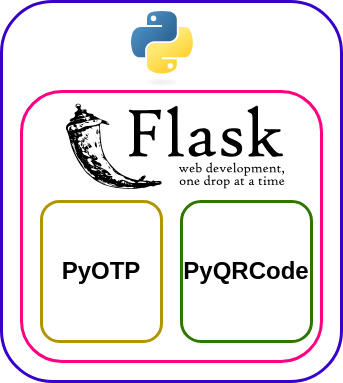
\includegraphics[width=4cm]{image/totp-server.drawio}
            \end{center}
        \end{columns}
        \bigbreak
        Le serveur doit fonctionner avec l'application Google Authenticator.
    \end{frame}


    \section{Licence CC}\label{sec:licence}

    \begin{frame}{Licence}{Licence Creative Commons}
        Support de cours sous licence Creative Commons BY-NC-ND~.
        \bigbreak
        Vous pouvez donc, partager, copier, distribuer le document.
        \bigbreak
        Attribution requise à PapIT SASU - Pas d’utilisation commerciale - Pas de modification
        \bigbreak
        \centering
        
\includegraphics[width=5cm]{image/by-nc-nd-logo}
    \end{frame}
\end{document}
